\documentclass[8pt]{beamer}
\usepackage{tikz}


\usepackage{lmodern}			% Usa a fonte Latin Modern
\usepackage[T1]{fontenc}		% Selecao de codigos de fonte.
\usepackage[utf8]{inputenc}		% Codificacao do documento (conversão automática dos acentos)
\usepackage{indentfirst}		% Indenta o primeiro parágrafo de cada seção.
\usepackage{color}				% Controle das cores
\usepackage{microtype} 			% para melhorias de justificação
\usepackage{graphicx}
% Required package
\usepackage{subcaption}
% ---
% Configurações de aparência do PDF final

%\usepackage[section]{algorithm}
%\usepackage[numbered]{algo}

\usepackage{xcolor}

\usepackage{mathtools}
\usepackage{booktabs}
\usepackage[portuguese]{babel}
\usepackage[brazilian,hyperpageref]{backref}	 % Paginas com as citações na bibl
\usepackage[alf]{abntex2cite}	% Citações padrão ABNT


%The used theme. Options: No page number, progress bar at the bottom
\usetheme[progressbar=foot]{metropolis}
\makeatletter
\setlength{\metropolis@progressinheadfoot@linewidth}{2pt}
\setlength{\metropolis@titleseparator@linewidth}{2pt}
\setlength{\metropolis@progressonsectionpage@linewidth}{2pt}

%Information to be included in the title page:
\title{Prova de conceito de um modelo classificador de áreas irregulares na Floresta Amazônica baseado em Transformers Visuais}


\author{Victor Moraes}
\institute{UFMG}
\date{\today}


\begin{document}

\frame{\titlepage}

\begin{frame}{Estrutura da Apresentação}
    \tableofcontents
    {\usebeamerfont{frametitle}\usebeamercolor[fg]{frametitle}Summary}

\end{frame}

\section{Introdução} 

    %Este trabalho estuda as limitações das técnicas já estabelecidas de redes convolucionais e realizará uma prova de conceito de uma técnica de visão computacional de arquitetura Swin para classificação de imagens de áreas irregulares da amazônia, baseado em transformers visuais. Assim como a comparação de desempenho dentre as duas técnicas. Além de prover uma metodologia e experimentos reprodutíveis para utilização da arquitetura Swin para problemas análogos, de diferentes conjuntos de dados de sensoriamento remoto.


\section{Motivação} 
\begin{frame}{Motivação}  

    \begin{figure}[!h]
    \centering
    \includegraphics[width=0.6\columnwidth]{Imagens/Ti-Munduruku-Foto_Marizilda_Cruppe_Amazônia_Real.jpg}
    \caption[width=0.2\columnwidth]{\\\small Garimpo ilegal na Terra Indígena Munduruku, município de Jacareacanga. Foto: Marizilda Cruppe/Amazônia Real}
    \label{fig:garimpo}
    \end{figure}

    % A Floresta Amazônica enfrenta um acumulo histórico de degradação, além de crescentes níveis de desmatamento e destruição de habidats, seja por agricultura, mineração, extração e pecuária ilegais. Para diagnisticar tais degradações sobre a imensa área que a floresta cobre, o instuturo nacional de pesquisas espaciais possui satélites que realizam o sensoriamento remoto da região, para diagnisticar utilizando vários espectros e áreas abrangentes. Contudo até então foram usados satélites de baixa resolução para o espectro visível. Recentemente O INPE conta com satélites do espectro visiível de altissimas resoluções e que combinados com técnicas de visão computacional e aprendizado profundo, podem diagnisticar com presição degradações esparças e de pequena escalas, ou mesmo ocultas.

\end{frame}

\section{Revisão Bibliográfica} 
\begin{frame}{Revisão bibliográfica }
\begin{itemize}
    \item Domínio do problema: Sensoriamento remoto
    \item Aprendizado de máquina
    \item Redes convolucionais
    \item Transformers
    \item Trabalhos anteriores
\end{itemize}

    % Neste capítulo, será apresentado inicialmente definições do domínio do problema de classificação e identificação de cenas em sensoriamento remoto na seção~\ref{sec:Cap2_dominio}, bem como suas características e contexto. Seguindo por um apanhado teórico da seção envolvendo aprendizado de máquina, redes neurais, redes neurais profundas, convolucionais e~\textit{transformers}, no que tange interseções com possíveis soluções para o problema. E por fim, na seção~\ref{sec:Cap2_revisao_literatura} uma revisão da literatura e do atual estado da arte no que tange o problema de classificação visual no que tange a sensoriamento remoto. Apresentando trabalhos que envolveram soluções tanto para o campo, quanto para implementações de redes neurais profundas.
\end{frame}


\begin{frame}{Revisão bibliográfica - Sensoriamento Remoto}
    \begin{figure}[!ht]
        \centering
        \includegraphics[width=0.6\columnwidth]{
            Imagens/instrutorgis\_sensoriamento\_remoto\_ilustracao.png
        }
        \caption{Sensoriamento remoto. Figura:\cite{InstrutorGIS}}
    \label{fig:sensoriamento}
    \end{figure}
    % O problema em questão, de identificação de regiões com garimpo em imagens de satélite, e pertencem ao campo de sensoriamento remoto. O sensoriamento remoto consiste em aquistar ou analisar medições de uma região geográfica terrestre, ou atmosférica. Podem ser realizadas por imagens aéreas ou por satélites, podendo abranger diferentes partes do espectro eletromagnético.Frequentemente consistem em métodos de aquisição ou processamento de sinais e imagens, para obter características ou reconhecer padrões em tais localidades~\cite{emery2017introduction}.O termo foi cunhado referir-se a medição realizada por algum meio indireto ou “remoto”, em vez de um contato direto com sensores no ambiente medido~\cite{emery2017introduction}.
    \end{frame}

\begin{frame}
\frametitle{Aprendizado de máquina - Definições}

\begin{quotation}
    
“Campo de estudos que visa a dar computadores a habilidade de aprender sem serem explicitamente programados para determinada tarefa." ~\cite{Samuel1959SomeSI}
\end{quotation}

\begin{quotation}
“Um algoritmo dito conseguir uma experiência E com respeito a determinada classe de tarefas T e com medidas de desempenho P, se seu desempenho nas tarefas em T, medidas por P, melhoram a partir da experiência E.” ~\cite{Mitchell97} 
\end{quotation}
% Aprendizado de máquina é um campo que estuda algorítimos capazes de aprender e realizar inferências a partir de dados. O termo foi cunhado em ~\cite{Samuel1959SomeSI}, como “Campo de estudos que visa a dar computadores a habilidade de aprender sem serem explicitamente programados para determinada tarefa.”.

%Já em~\cite{Mitchell97} define um algorítimo de aprendizado como “Um algoritmo dito conseguir uma experiência E com respeito a determinada classe de tarefas T e com medidas de desempenho P, se seu desempenho nas tarefas em T, medidas por P, melhoram a partir da experiência E.”

\end{frame}


\begin{frame}{Aprendizado de máquina - Exemplo}
    Exemplo:  

    \begin{itemize}
        \item Tarefa T: Problema de classificação
        \item Experiência E: Amostras dentre k classes a classificar
        \item Desempenho P: acurácia do algorítimo
    \end{itemize}
    
    Produzir função:

    \(f:\Re^n\rightarrow \{1,\ldots,k\}\). Quando \( y=f(x) \)
    %Para melhor entender cada constituinte dessa definição, podemos utilizar de um exemplo. A tarefa T temos como exemplo o problema de classificação, que consiste do algorítimo responder quais das k categorias para o qual ele experimentou em E, certas amostras de entradas pertencem. Para resolver tal tarefa, tal algorítimo de aprendizado deve produzir uma função \(f:\Re^n\rightarrow \{1,\ldots,k\}\). Quando \( y=f(x) \), o modelo atribui uma entrada descrita pelo por \(x\), que nosso caso constitui uma amostra de entrada, a uma categoria identificada por um código numérico \(y\). Uma variante do mesmo problema é em vez de classificar qual classe, retornar a distribuição de probabilidade sobre as classes~\cite{GoodBengCour16}. A medida de desempenho P, necessária para avaliar as habilidades de um dado algorítimo. Tal medida de desempenho é geralmente atrelada ao tipo de tarefa sendo realizada pelo sistema. 
    \end{frame}


\begin{frame}
        \frametitle{Métricas de desempenho}
        \begin{figure}[!ht]
            \centering
                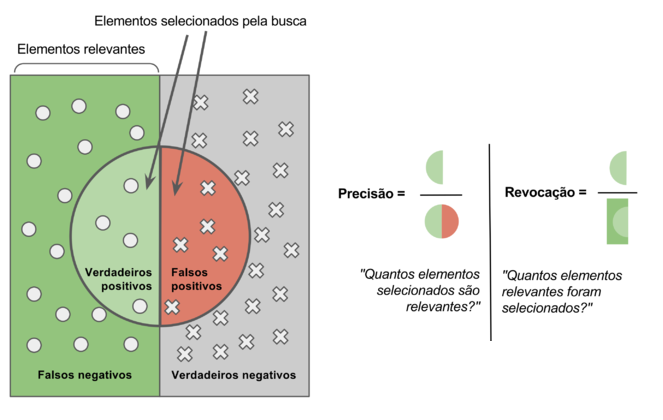
\includegraphics[width=0.7\columnwidth]{Imagens/Precisão_e_revocação_cropped.png}
            \caption{Ilustração das métricas de precisão e revocação. Fonte: WikiCommons}         
        \end{figure}
\end{frame}  


\begin{frame}{Métricas de desempenho}
    \begin{figure}[!ht]
        \centering
            \includegraphics[width=0.6\columnwidth]{Imagens/matrix_confusão.png}
            \begin{equation} P = \frac{VP}{VP + VP} \end{equation}
            \begin{equation}R = \frac{VP}{VP + FP}\end{equation}
            \begin{equation}AC = \frac{VP + VN}{VP + VN + FM + FP}\end{equation}
        \caption{Matriz Confusão, Equações de Precisão, Revocação e Acurácia}         
    \end{figure}
\end{frame}

\begin{frame}{Métricas de desempenho}
    \begin{figure}[!ht]
        \centering
        \begin{equation}F_1 = \frac {P \times R}{P + R}\end{equation}
            \begin{equation}F_\beta = (1+\beta^2) \times \frac {P \times R}{\beta^2 P + R}\end{equation}
            \begin{equation}F_2 = 5 \times \frac {P \times R}{5 P + R}\end{equation}    
        \caption{Equações de $F_\beta$ e $F_2$}         
    \end{figure}
\end{frame} 

\begin{frame}{Curva PR}
    \begin{figure}[!ht]
        \centering
        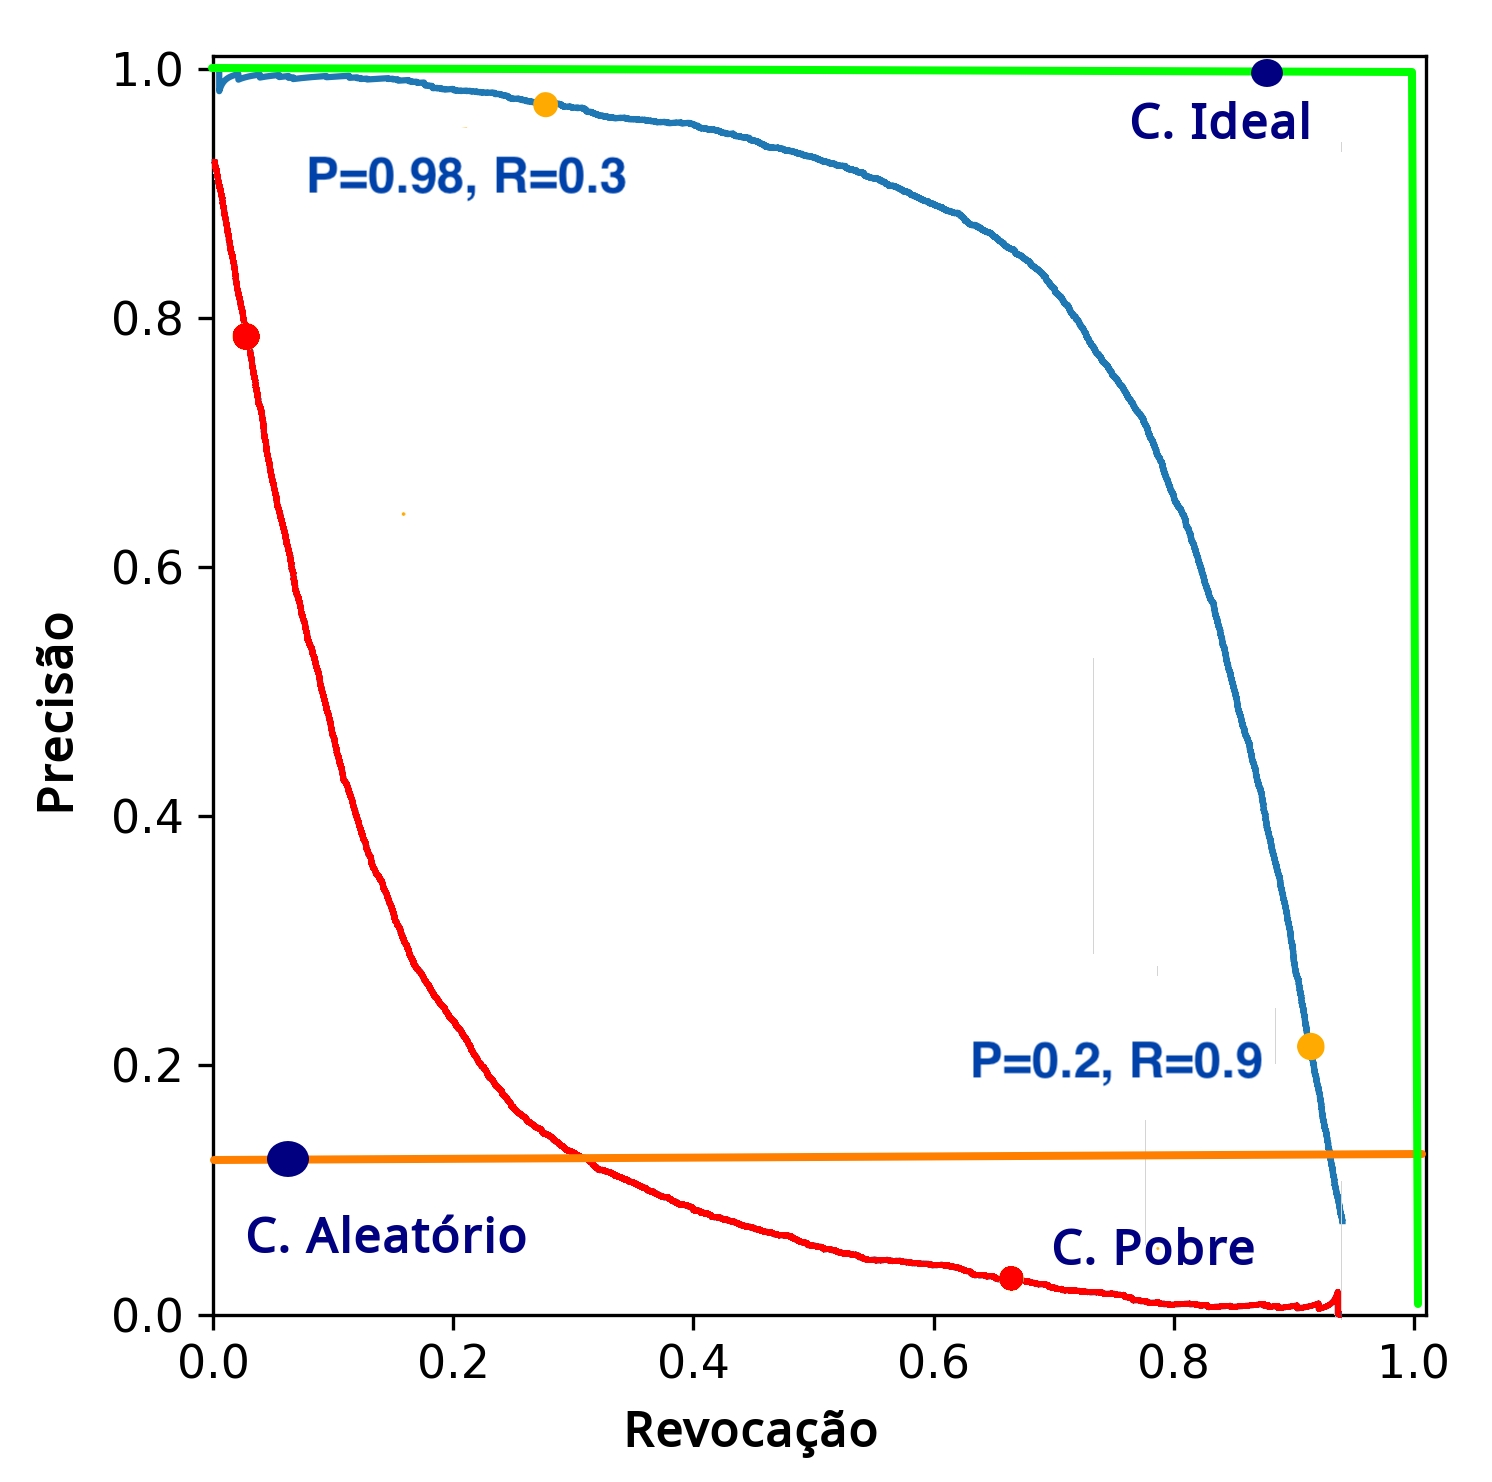
\includegraphics[width=0.5\columnwidth]{Imagens/pr_curve_orig.jpg}
        \caption{Curva Precisão-Recisão}
    \end{figure}
\end{frame}  

\begin{frame}{Regressão logística}
    \begin{figure}[!ht]
        \centering
        \begin{minipage}[c]{0.4\textwidth}
            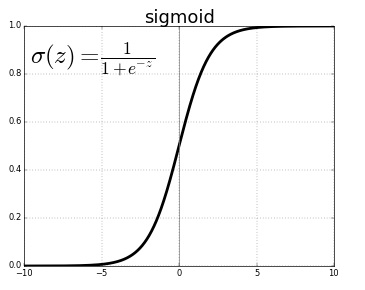
\includegraphics[width=\columnwidth]{Imagens/sigmoid-activation-function.jpg}
        \end{minipage}%
        \begin{minipage}{0.5\textwidth}
            \begin{equation} \sigma(x) = \frac{1} {1+ exp(-z(x))}\end{equation}
        \end{minipage}       
        \label{fig:sigmoid}
        \caption{Função de ativação \textit{Sigmoid}.}
    \end{figure}
% A regressão logística é uma técnica estatística que tem como objetivo produzir, a partir de um conjunto de observações, um modelo que permita a predição de valores tomados por uma variável categórica, frequentemente binária, a partir de uma série de variáveis explicativas contínuas e/ou binárias
\end{frame}

\begin{frame}{Otimização}

\begin{equation}
    w \leftarrow w - \eta \nabla L(w)
\end{equation}
\begin{equation}
Q(w) = \frac{1}{n}\sum_i Q_i(w)\;\;\;\;\implies\;\;\;\; \nabla Q(w) = \frac{1}{n}\sum_i \nabla Q_i(w)
\end{equation}
\begin{figure}[!ht]
    \centering
        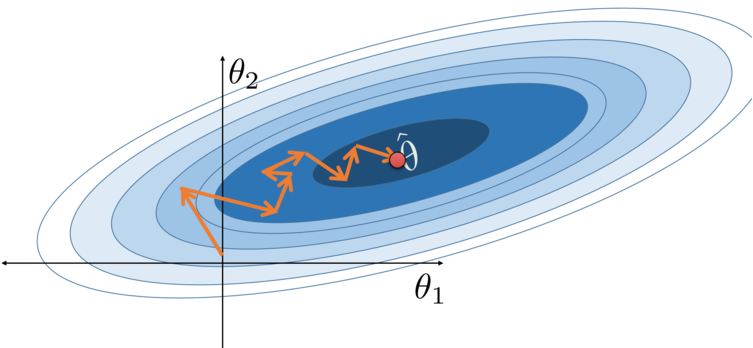
\includegraphics[width=0.6\columnwidth]{Imagens/stochastic_gradient_descent.PNG}
    \caption{Ilustração do algorítimo gradiente descendente estocástico. }
    \label{fig:SGD}
\end{figure}
\end{frame}

\begin{frame}{Função de perda}

    \begin{equation}
        ECB(y_c) = -\sum_{c=0}^{M} y_c \times log(\hat{y_c})
    \end{equation}

    \begin{equation}
        Focal(y_c) = -\sum_{c=0}^{M} (1-w_i \times y_c)^\gamma \times log(\hat{y_c})
    \end{equation}
% Otimizadores possuem como objetivo ajustar pesos de uma função de custo para minimizar ou maximizar tal custo. Para quantificar o custo são utilizadas métricas de perda. Dentre elas, as funções de custos ideais para classificação binária multiclasses e multirótulos temos a entropia binária cruzada, definida por

% Para conjuntos de dados muito desbalanceados, pode-se mitigar o sobre-ajuste da classe dominante utilizando BCE com pesos do inverso da frequência das classes:    
\end{frame}




\begin{frame}{Redes Neurais Artificiais Profundas}

    \begin{figure}[!ht]
        \centering
        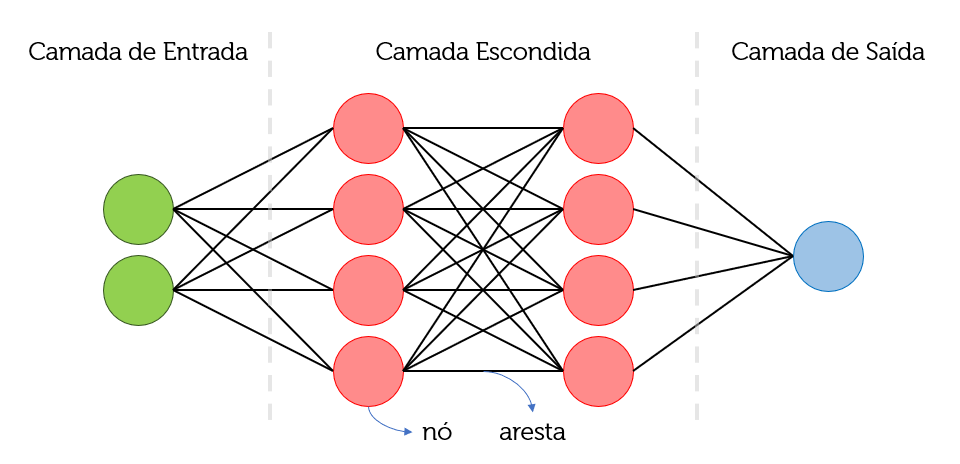
\includegraphics[width=0.6\columnwidth]{
            Imagens/RedeNeural.PNG
        }
        \caption{Exemplo de uma rede de perceptrons de multiplas camadas - MLP.}
        \label{fig:ann}
    \end{figure}
% O termo redes neurais profundas e o aprendizado profundo, ou comumente chamado de \textit{deep learning}, se refere a redes neurais artificiais com múltiplas camadas ocultas. Foram uma das tecnologias maior desenvolvidas nos últimos anos, e se tornaram cada vez mais popular. Devido a sua superior \textit{performance} em extração de características, teve sucesso por distintos domínios, como visão computacional, reconhecimento de fala, processamento natural de linguagem e em big data.

%Um dos riscos envolvendo o treinamento de redes neurais profundas é o problema de \textit{overfiting}\footnote{Sobre-ajuste}. Se trata de quando o modelo é treinado e para gerar uma função próxima demais aos dados de treino, e perdem generalidade, falhando em predições em dados fora do conjunto de treino. Para mitigar o surgimento de \textit{overfiting} durante o treino, são utilizadas técnicas de regularização. Consistem em adicionar penalidade à complexidade do modelo, de forma que o treino otimize para se tornar uma função genérica. Dentre as técnicas de regularização possíveis de DNNs\footnote{\textit{Deep Neural Networks}}, podemos citar o \textit{Dropout, Dropconnect e pruning}, que consistem em respectivamente a remoção, adição de conexão entre neurônios e remoção de neurônios~\cite{hastie01statisticallearning}.        
\end{frame}


\begin{frame}{Redes convolucionais}
        \begin{figure}[!ht]
            \centering
            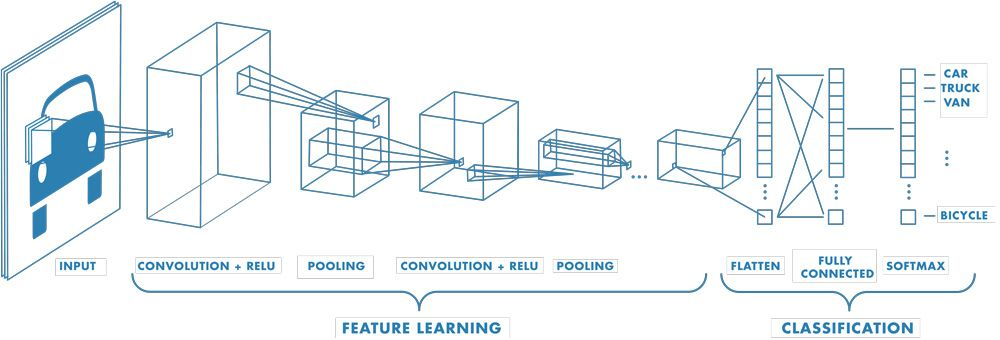
\includegraphics[width=0.95\columnwidth]{
                Imagens/CNN_mathworks.jpg
            }
            \caption{Arquitetura de uma rede convolucional. }
            % Filtros extratores de características são aplicados em diferentes resoluções e campos visuais. A saída de cada imagem convoluta alimenta a próxima camada. As ultimas camadas completamente conectadas realizam a classificação.
            \label{fig:cnn}
        \end{figure}


% Uma arquitetura clássica é a rede neural convolucional (CNN\footnote{\textit{Convolutional Neural Network}}), que utiliza convoluções para extrair características de uma imagem entre cada camada de filtros. Também possui camadas de \textit{pooling}, não lineares e camadas completamente conectadas~\cite{8308186}. Uma dos pressupostos das \textit{CNNs} é os filtros serem indiferentes a translações das características na imagem, possibilitando assim uma eficiente extração de características para composição e identificação da imagem.


%Em 2012, o modelo de CNN AlexNet ultrapassou em desempenho os modelos do estado da arte em uma grande margem. Dois fatores promoveram tal degrau de evolução: a disponibilidade de grandes \textit{datasets}\footnote{Conjunto de dados} como o ImageNet e a comoditização de placas gráficas, que promoveram significativamente mais poder computacional para treino, já que são aceleradores de operações vetorizadas e sobre matrizes. Dessa forma, desde 2012 CNNs se tornaram o modelo padrão para tarefas de visão computacional \cite{alom2018history}.

%A maior vantagem dos modelos CNN em comparação com os métodos anteriores era de conseguir ser treinados ponta a ponta, sem a necessidade de criação de filtros ou a criação manual de extratores de características visuais. Também possuem duas importantes propriedades como invariância translacional, isto é, o sistema produz a mesma resposta independente de translação; e campo receptivo restrito, o que significa que neurônios das primeiras camadas capturam detalhes finos e locais.
\end{frame}


\begin{frame}{Redes convolucionais}
    
    \begin{figure}[!ht]
        \centering
            \begin{minipage}{0.45\textwidth}
                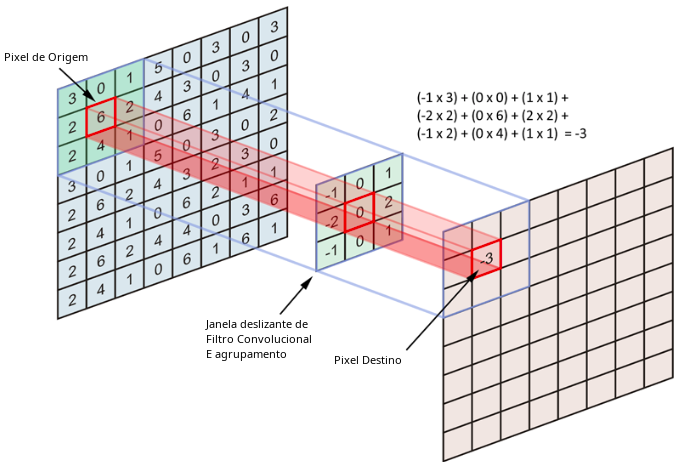
\includegraphics[width=\columnwidth]{Imagens/operacao_conv.png}
                \caption{Operação de janela deslizante aplicando operações de convolução e pooling.}
            \end{minipage}
            \begin{minipage}{0.45\textwidth}
                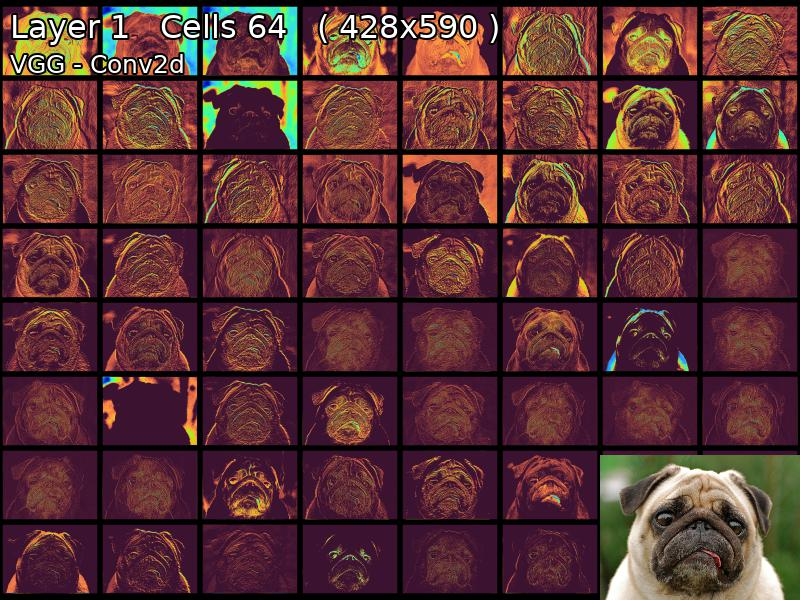
\includegraphics[width=\columnwidth]{Imagens/mapextrackt.jpg}
                \caption{Biblioteca Pytorch de visualização de filtros extratores.}
            \end{minipage}
            %\label{fig:conv}
        \end{figure}  
        
% --- Source: https://towardsdatascience.com/applied-deep-learning-part-4-convolutional-neural-networks-584bc134c1e2

% Uma arquitetura clássica é a rede neural convolucional (CNN\footnote{\textit{Convolutional Neural Network}}), que utiliza convoluções para extrair características de uma imagem entre cada camada de filtros. Também possui camadas de \textit{pooling}, não lineares e camadas completamente conectadas~\cite{8308186}. Uma dos pressupostos das \textit{CNNs} é os filtros serem indiferentes a translações das características na imagem, possibilitando assim uma eficiente extração de características para composição e identificação da imagem.


%Em 2012, o modelo de CNN AlexNet ultrapassou em desempenho os modelos do estado da arte em uma grande margem. Dois fatores promoveram tal degrau de evolução: a disponibilidade de grandes \textit{datasets}\footnote{Conjunto de dados} como o ImageNet e a comoditização de placas gráficas, que promoveram significativamente mais poder computacional para treino, já que são aceleradores de operações vetorizadas e sobre matrizes. Dessa forma, desde 2012 CNNs se tornaram o modelo padrão para tarefas de visão computacional \cite{alom2018history}.

%A maior vantagem dos modelos CNN em comparação com os métodos anteriores era de conseguir ser treinados ponta a ponta, sem a necessidade de criação de filtros ou a criação manual de extratores de características visuais. Também possuem duas importantes propriedades como invariância translacional, isto é, o sistema produz a mesma resposta independente de translação; e campo receptivo restrito, o que significa que neurônios das primeiras camadas capturam detalhes finos e locais.
\end{frame}


\begin{frame}{ResNet}

    \begin{figure}[!ht]
        \centering
        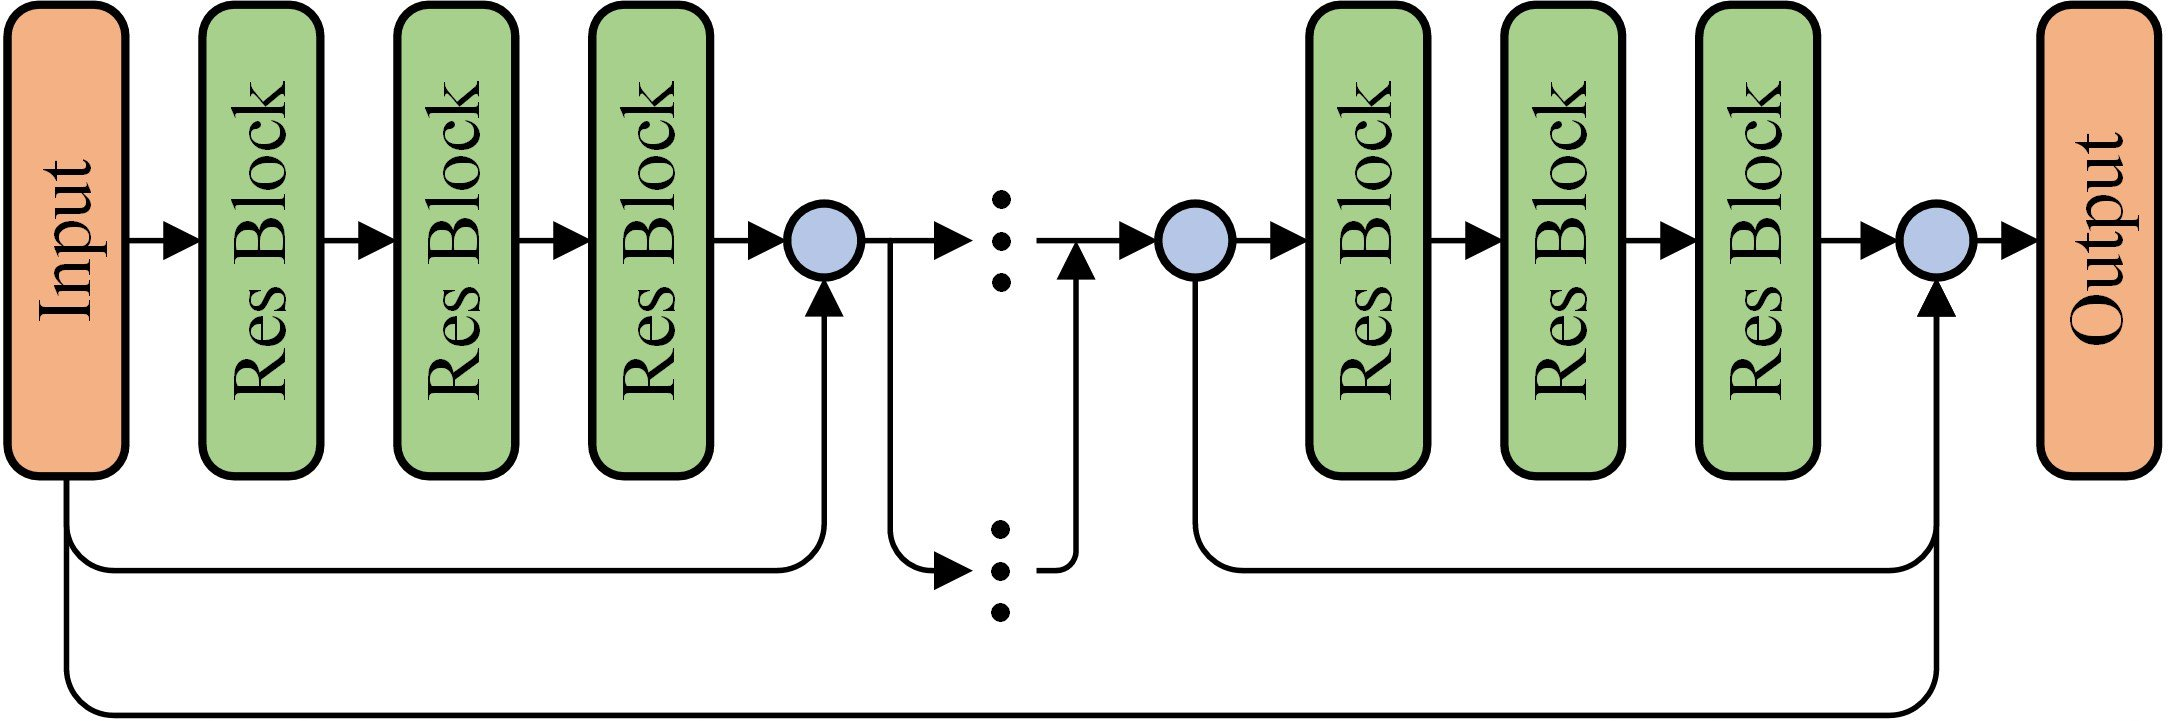
\includegraphics[width=0.9\columnwidth]{Imagens/An-illustration-of-the-deep-residual-network-ResNet-structure-More-shortcut.jpg}
        \caption{ Arquitetura redes ResNet.}
       \label{fig:ResNet-Rsp}
    \end{figure}
% Um dos principais desafios envolvido o treino de \textit{CNNs} aplicado a sensoriamento remoto é representar um estado de características que cubram as variações fotográficas, tanto em características do sensor, como variações da imagem no dia, clima, estação e plataforma da câmera, o que se torna uma tarefa difícil. Para uma localização efetiva, o modelo deve ser robusto a todas essas variações, que requer um grande conjunto de treino que cobre boa parte das diversas condições possíveis. Tal conjunto de dados não é disponível e nem viável de obter, pois se trata um volume muito grande de amostras. Tais limitações levam a necessitar o desenvolvimento de algorítimos que aprendem seletivamente para que o poder computacional seja utilizado eficientemente, bem como reutilizar conhecimento prévio e evitar treinamento redundante~\cite{rostami2019learning}.  Dentre as técnicas utilizadas para implementar esses modelos mais eficientes, temos como exemplo o aprendizado supervisionado fraco, e a transferência de aprendizado.    
\end{frame}


\begin{frame}{Transformer Visual}

    \begin{figure}[!ht]
        \centering
        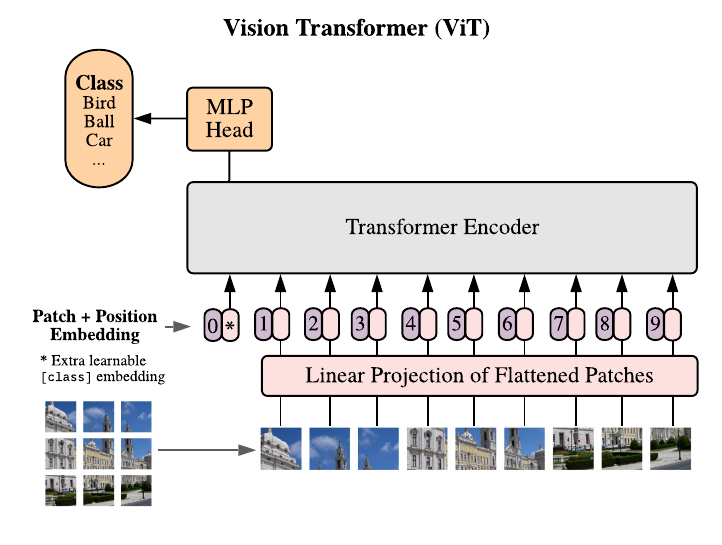
\includegraphics[width=0.7\columnwidth]{
            Imagens/vit.png
        }
        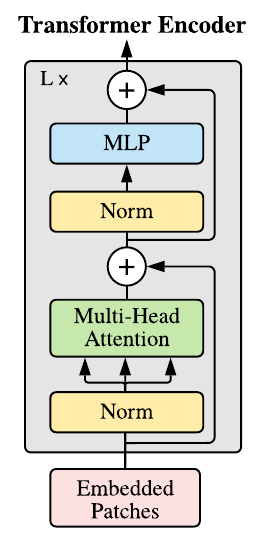
\includegraphics[width=0.2\columnwidth]{
            Imagens/encoder.png
        }
        \caption{\cite{dosovitskiy2020image}}
        % O ViT divide uma imagem em uma grade de recortes quadrados, cada fragmento é achatado em um vetor único contendo todos os canais de todos os pixeis, e projetando-os em uma dimensão de entrada desejada, alimentando a camada de múltiplos Encoders em paralelo. 
        \label{fig:vit}
    \end{figure}
\end{frame}


\begin{frame}{Auto-Atenção}

    \begin{figure}[!ht]
        \centering
        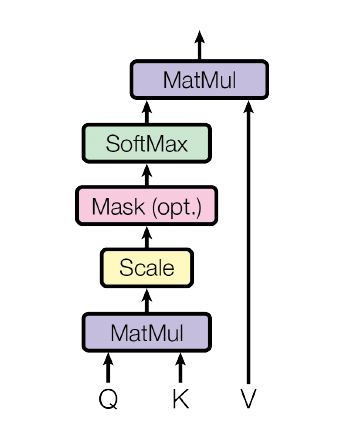
\includegraphics[width=0.3\columnwidth]{
            Imagens/Scaled Dot-Product Attention.png
        }
        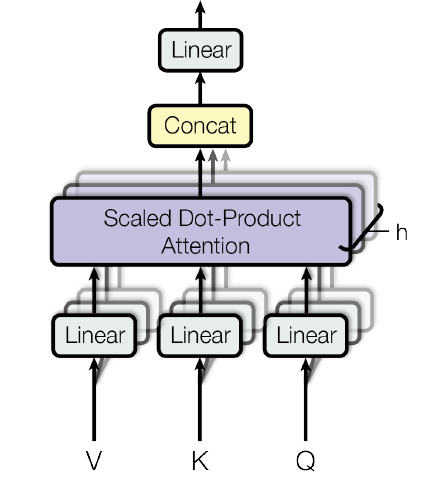
\includegraphics[width=0.3\columnwidth]{
            Imagens/Multi-Head Attention.png
        }

        \begin{equation}
            Y = softmax(QK^T)V
        \end{equation}
        \caption{\cite{dosovitskiy2020image}}
        % O ViT divide uma imagem em uma grade de recortes quadrados, cada fragmento é achatado em um vetor único contendo todos os canais de todos os pixeis, e projetando-os em uma dimensão de entrada desejada, alimentando a camada de múltiplos Encoders em paralelo. 
        \label{fig:vit}
    \end{figure}
\end{frame}

\begin{frame}{Transformer Swin}

    \begin{figure}[!ht]
        \centering
        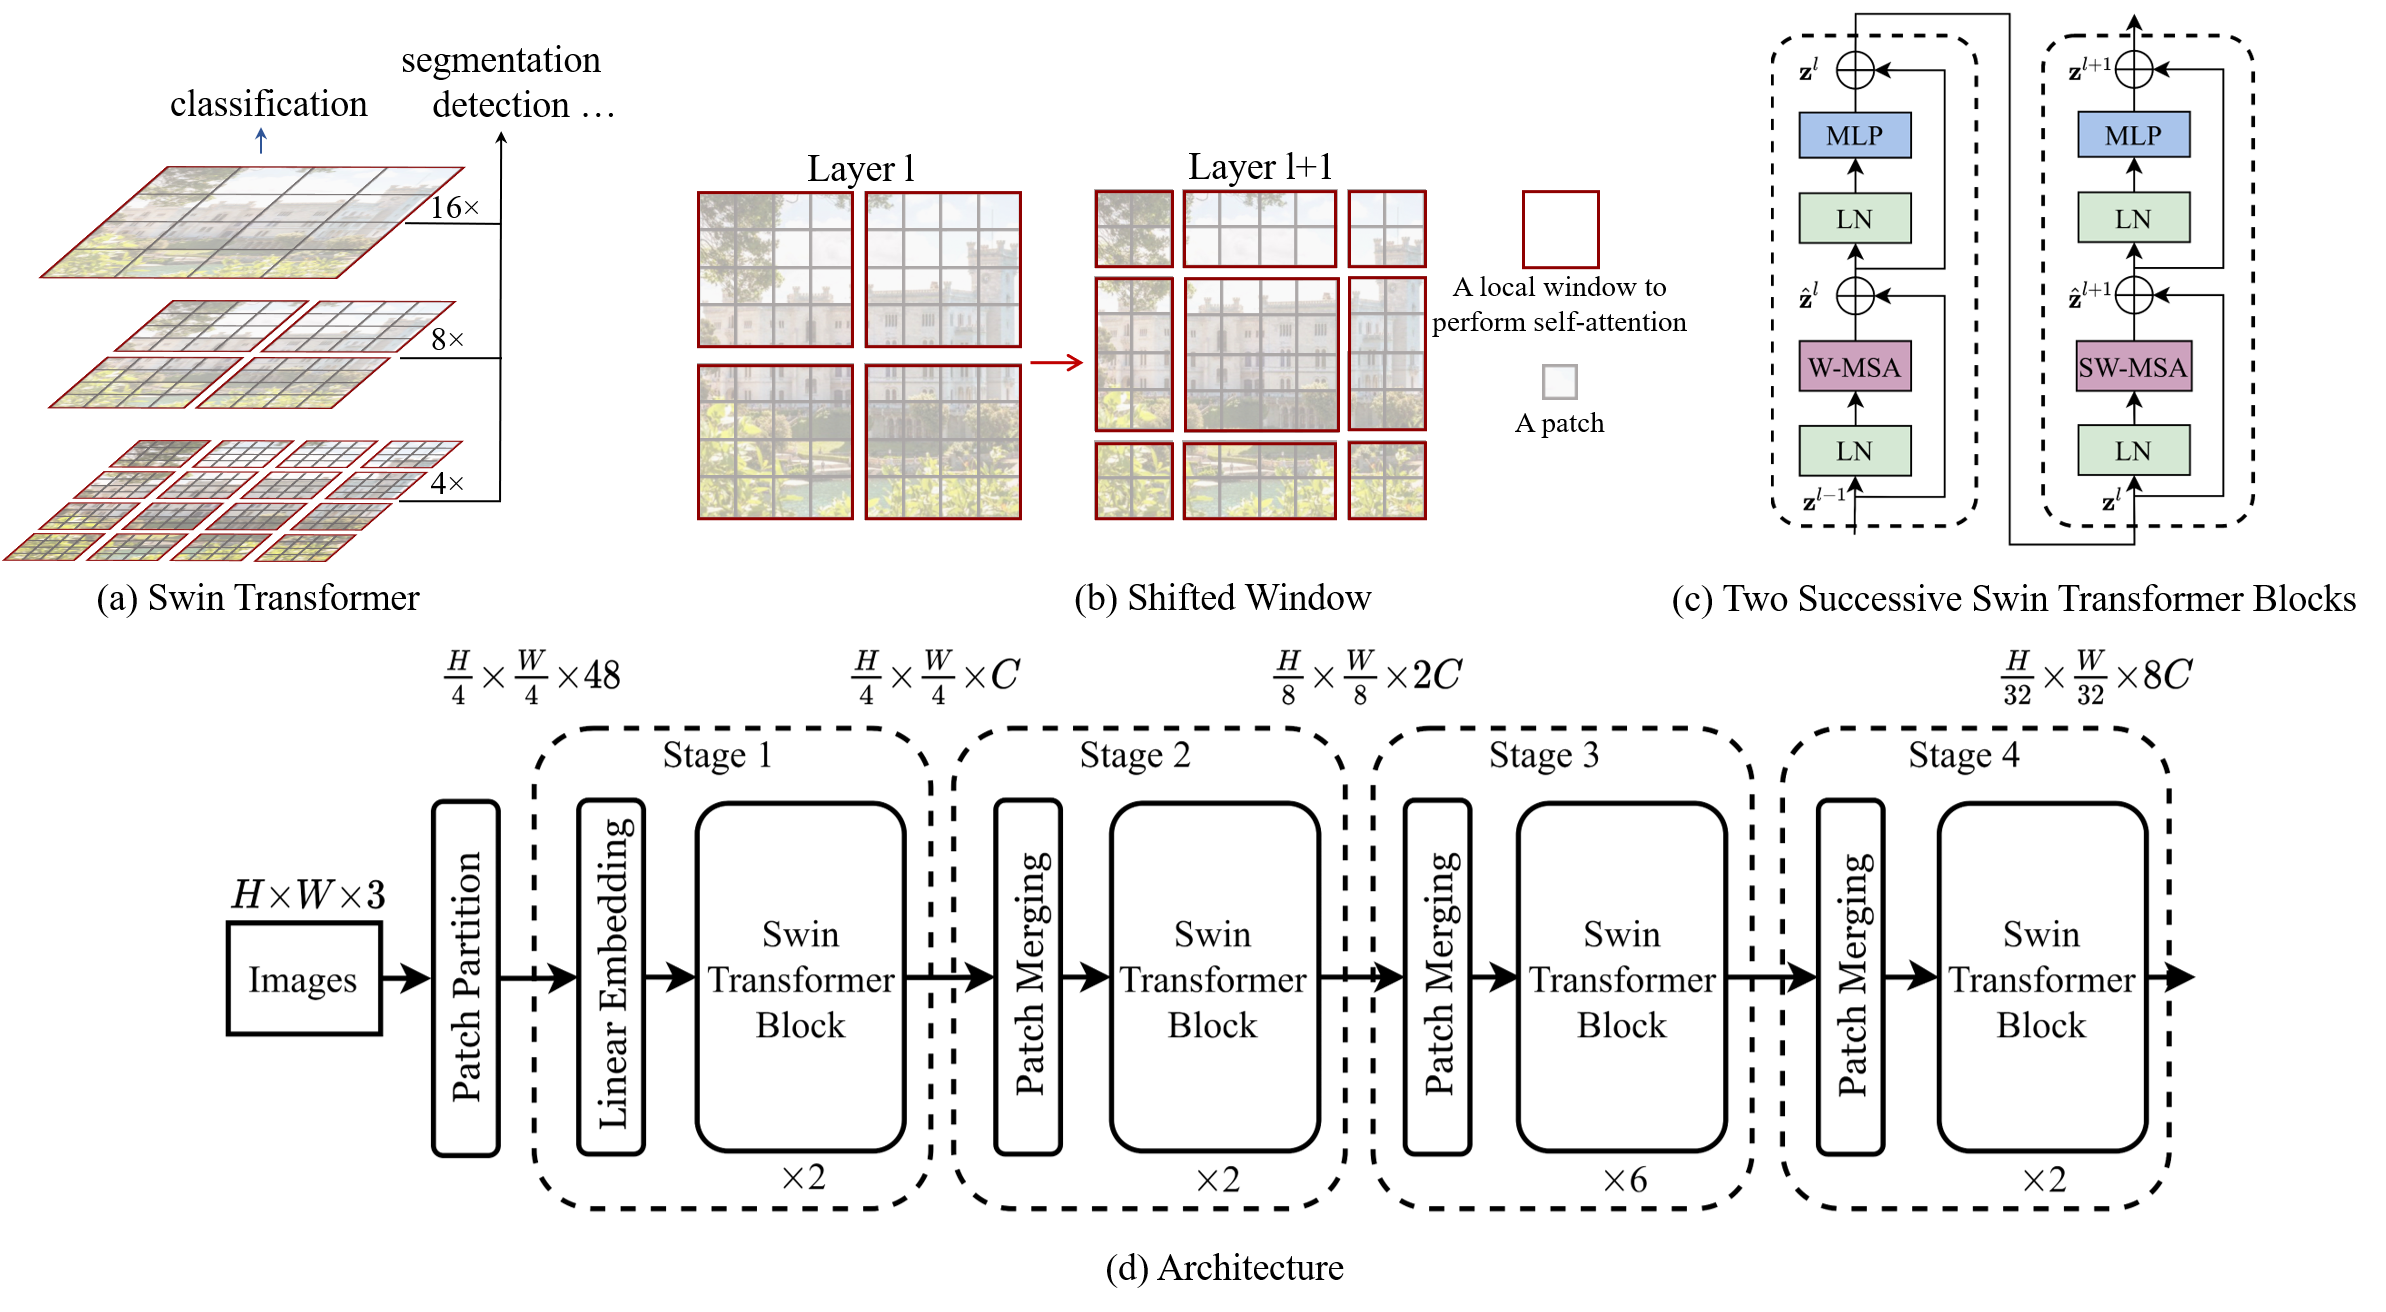
\includegraphics[width=\columnwidth]{Imagens/arquitetura swin.png}
        \caption{Arquitetura Swin (\textit{Shifted-Window} - Janela deslocada) ~\cite{liu2022swin}}
        \label{fig:SWIN-arquitetura}
    \end{figure}

    % Em~\cite{liu2022swin} foi proposto uma arquitetura de transformer visual com melhorias capazes de reduzir o custo computacional do cálculo de atenção entre cada recorte da imagem de entrada. Este trabalho aponta que a ordem de complexidade do ViT clássico é $O(n^2)$, sendo $n$ o número de retalhos, já que é calculado a métrica de atenção entre cada retalho com todos os outros demais. Com isso, torna caro o treino para maiores resoluções ou granularidade de detalhes. A arquitetura Swin, ou \textit{Shifted Window} se baseia em uma disposição hierárquica de Transformers, como ilustra a figura \ref{fig:SWIN-arquitetura}, sendo que nas camadas mais baixas, coletam atenção apenas localmente e não com todo restante da imagem. Dessa forma o custo se torna aproximadamente linear. 
\end{frame}

\begin{frame}{Trabalhos anteriores}

    \begin{itemize}
        \item Detecção de mudanças para detecção de minas de ouro \cite{rs14071746}
        \item Classificação de minas e represas \cite{s20236936}
        \item Dataset MillionAID e transformers visuais ~\cite{wang2022empirical}
        \item transformers visuais para detecção de desmatamento ~\cite{9701667}
    \end{itemize}
\end{frame}

\section{Metodologia} 

\begin{frame}

\frametitle{Método}

\begin{figure}[!ht]
    \centering
    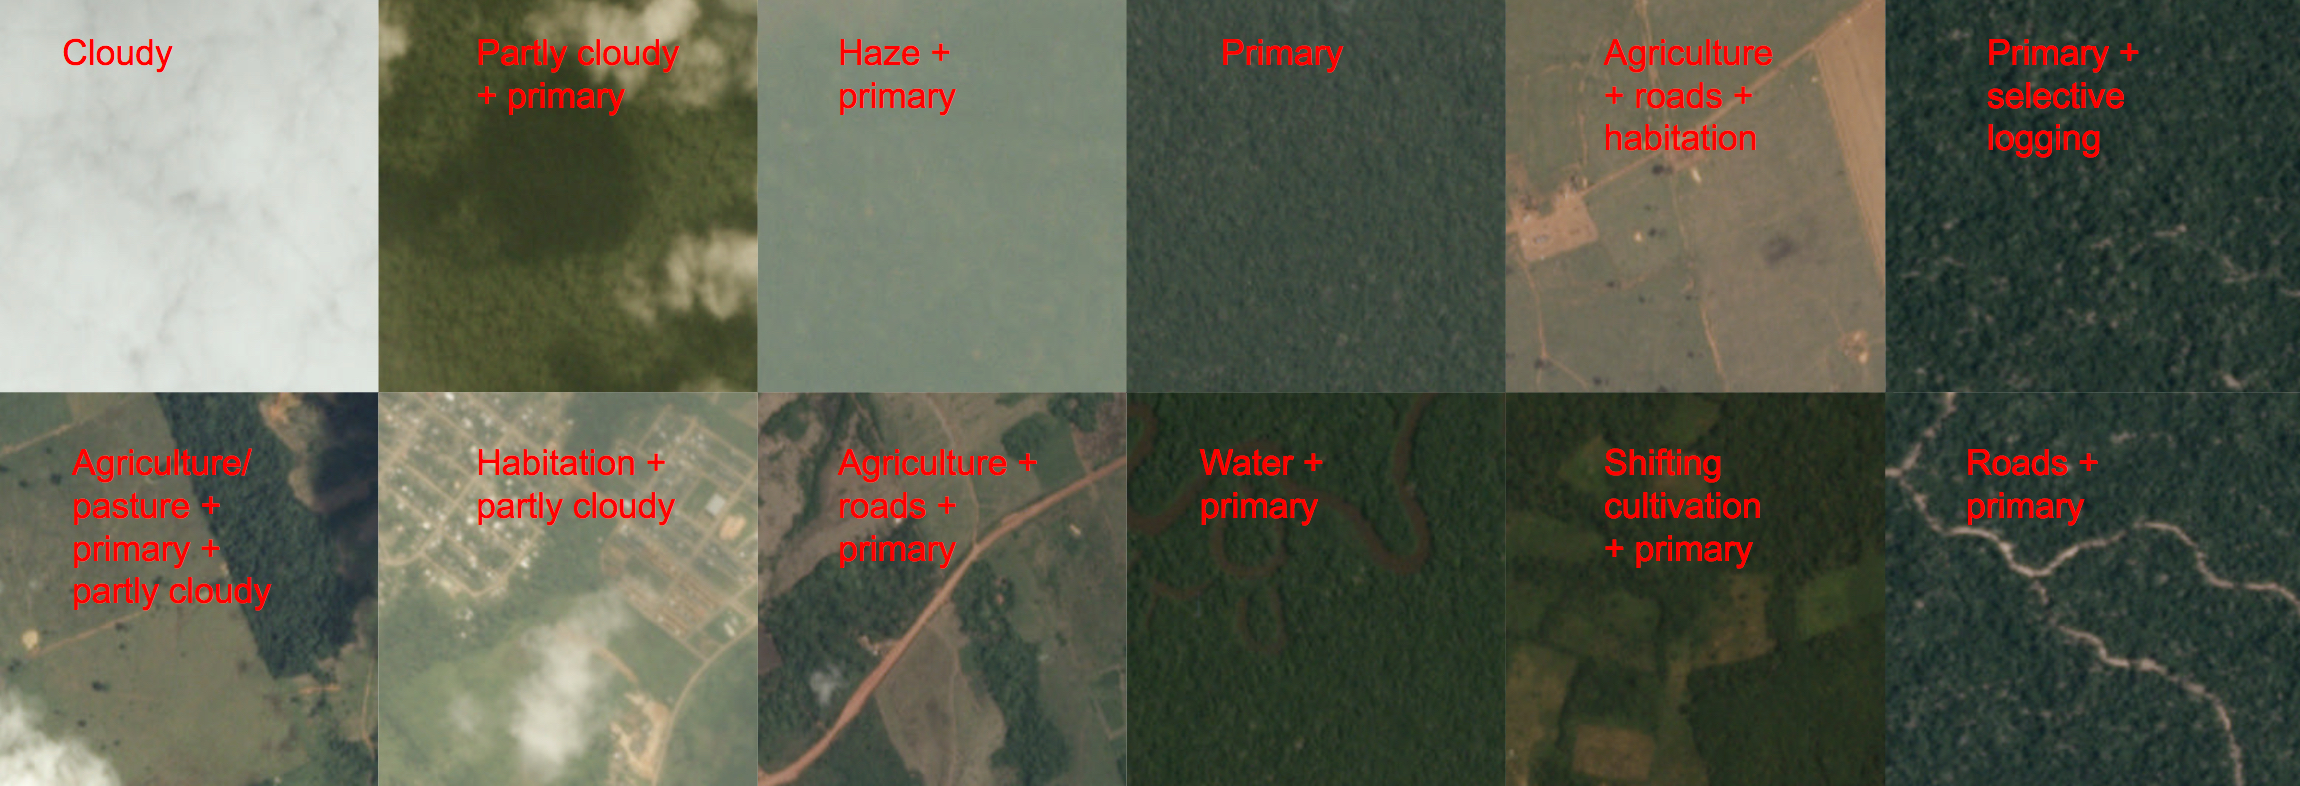
\includegraphics[width=0.9\columnwidth]{
        Imagens/chips.jpg
    }
    \caption{Amostras de classes do dataset Amazônia do Espaço Fonte:\cite{Kaggle:PlanetAmazonFromSpace}}\label{fig:dataset}
\end{figure}
 
% Este conjunto de dados é de imagens coletados dos satélites Planet Flock entre 2016 e 2017. Todas as imagens são da bacia amazônica. Este data set concerne ao desmatamento e cobrindo condições atmosféricas, coberturas de terreno e fenômenos raros. Cada amostra é um recorde de $256 \times 256$ pixeis RGB, pertencente a uma ou mais das 17 classes distintas e possui resolução espaciais variáveis, por exemplo, de $3 m$ por píxel. Este data set foi publicado pela empresa Planet\footnote{https://www.kaggle.com/c/planet-understanding-the-amazon-from-space/data} na plataforma Kaggle, de concursos de aprendizado de máquina. Também são disponibilizadas o mesmo conjunto de dados com o canal de infravermelho-próximo e sem compressão.

% Outros datasets também foram considerados mas por limitaões de tempo e de tratamento das amostras não foram possíveis de serem utilizadas
\end{frame}



\begin{frame}{Premissas e proposta de solução}
    \begin{itemize}
        \item Explorar viés indutivo dos transformers visuais
        \item Comparar desempenho de um modelo Swin e ResNet
    \end{itemize}
    
\end{frame}


\begin{frame}{Ambiente e ferramentas}
    \begin{itemize}
        \item Jupyter e ambiente cloud Google Collab
        \item Pytorch, SciKitLearn e NumPy
    \end{itemize}
% O Ambiente dos experimentos será em cadernos \textit{Jupyters}, para ser facilmente replicável e ser executável em nuvem, com a possibilidade de alugar recursos computacionais da plataforma em nuvem \textit{Google Colab}.



% Foram dispostos 100h de orçamento de recursos computacionais, em uma instância da plataforma com GPU NVidia Tesla T4 de 12 GB de RAM. CPU Intel(R) Xeon(R) CPU @ 2.20GHz, 12 GB de memória. Para o treinamento de redes neurais profundas, aceleradores como placas gráficas podem resultar em ganhos de tempo de até 40x em comparação com treinamentos em CPU, bem como o uso da RAM para placa gráfica para realizar \textit{caching}\footnote[1]{Caching é o processo de utilizar um espaço de memória para o armazenamento temporário e de acesso rápido de dados que possuem uma grande probabilidade de serem utilizados novamente} obtendo melhores tempos de acesso durante carregamentos. Todos resultados de experimentos serão executados neste \href{https://colab.research.google.com/github/vic-torr/thesis-experiments/blob/main/experiments/rsp_Swint_t_planet_portugues.ipynb}{Caderno Jupyter}.

% Pytorch é um \textit{framework}\footnote{Ferramental} de processamento de tensores e acelerados por GPU\footnote[3]{Unidade de Processamento Gráfico, Trad.:\textit{Graphic Process Unit}} ou TPUs \footnote{Unidade de Processamento de Tensores. Trad. de \textit{Tensor Processing Unit}} para aprendizado de máquina profundo. É código-aberto, possuindo um front-end de fácil utilização em Python, implementado em linguagens C++ e CUDA para otimizações de computações numéricas, matriciais e de diferenciação, extensivas para esta aplicação.
\end{frame}

\begin{frame}{Experimentos}
    \begin{enumerate}
        \item   Análise exploratória dos dados.
        \item   Pre-processamento do conjunto de dados e de carregadores de amostras.
        \item   Elaborar um modelo base.
        \item   Utilizar pesos do dos trabalhos disponibilizados para fine-tune. 
        \item   Elaborar modelo proposto baseado em transformers visuais.
        \item   Fixar os hiperparâmetros e metodologia de treino para modelos base e proposto e treiná-los novamente a fim de realizar comparações.
        \item   Análise dos resultados de ambos comparando desempenho em métricas relevantes ao problema.
        \end{enumerate}
        
\end{frame}
\subsection{Análise exploratória}
\begin{frame}{Análise exploratória}
        %\caption{Proporção de Classes do conjunto de dados \textit{Planet}}
        %\centering
    \begin{tabular}{*{4}{c}}
        \hline
        Classe                  &            Rótulo &  Amostras      &  Proporção (\%) \\
        \hline
        Mina Convencional       & conventional mine &        100     &       0,247 \\
        Roça de Ventos          &         blow down &        101     &       0,250 \\
        Queimada                &        slash burn &        209     &       0,516 \\
        Florescimento           &          blooming &        332     &       0,820 \\
        Garimpo                 &    artisinal mine &        339     &       0,837 \\
        Desmatamento Seletivo   & selective logging &        340     &       0,840 \\
        Área Descoberta         &       bare ground &        862     &       2,129 \\
        Nublado                 &            cloudy &       2089     &       5,161 \\
        Névoa                   &              haze &       2697     &       6,663 \\
        Habitação               &        habitation &       3660     &       9,042 \\
        Cultivação              &       cultivation &       4547     &      11,233 \\
        Parcialmente Nublado    &     partly cloudy &       7261     &      17,938 \\
        Águas                   &             water &       7411     &      18,308 \\
        Estrada                 &              road &       8071     &      19,939 \\
        Agricultura             &       agriculture &      12315     &      30,423 \\
        Clima Limpo             &             clear &      28431     &      70,236 \\
        Vegetação Primária      &           primary &      37513     &      92,673 \\
        \hline
    \end{tabular}
    %\label{table:proporcao_classes}
  
\end{frame}


\begin{frame}{Amostragem de cada classe}
    \begin{figure}[!ht]
        \centering
        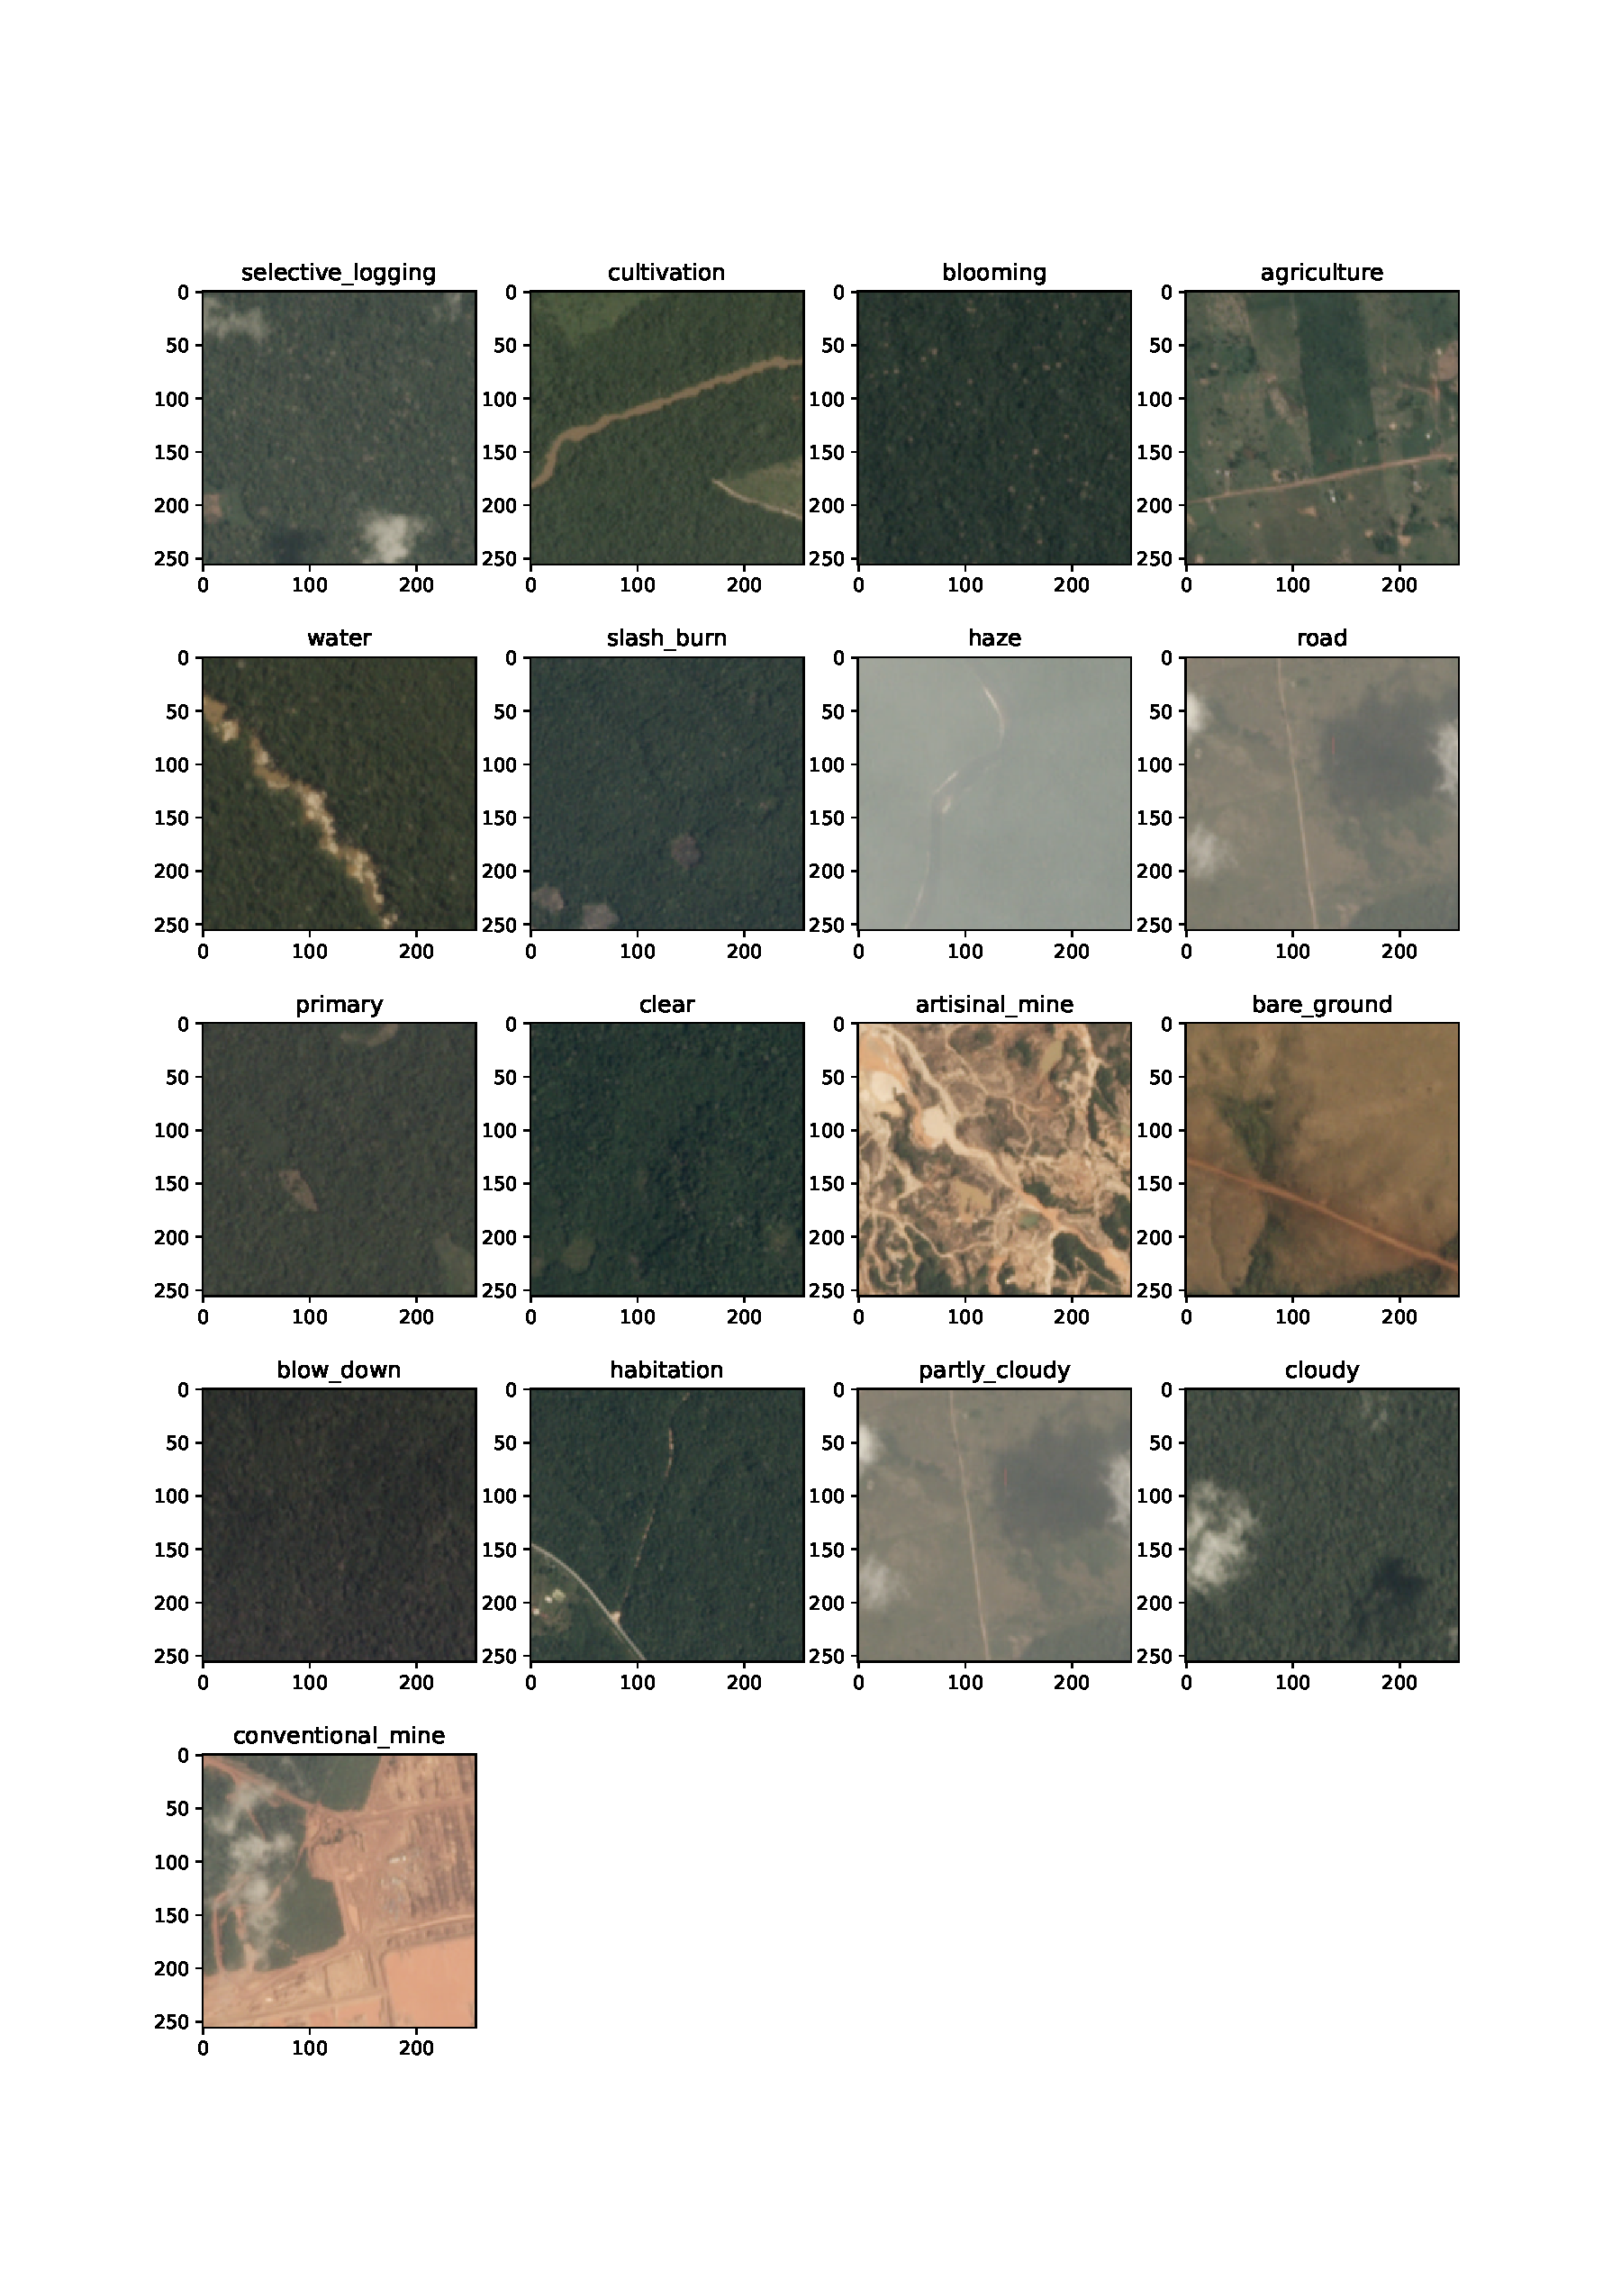
\includegraphics[width=0.7\textheight]{Imagens/results/rsp-resnet-50_planet_pt/Amostras de cada classe.pdf}
        \caption{Amostragem de cada classe de rótulo.
        Fonte: Autor}
       \label{fig:classes}
    \end{figure}
        
\end{frame}
    

\begin{frame}{Matriz de co-ocorrência}
    \begin{figure}[!ht]
        \centering
        \includegraphics[width=0.6\columnwidth]{Imagens/results/rsp-resnet-50_planet_pt/Matriz de Co-ocorrência.pdf}
        \caption{Matriz de co-ocorrência.
        Fonte: Autor}
       \label{fig:coocorrencia}
    \end{figure}    
\end{frame}


\begin{frame}{Agrupamento de amostras}
    \begin{figure}[!ht]
        \centering
        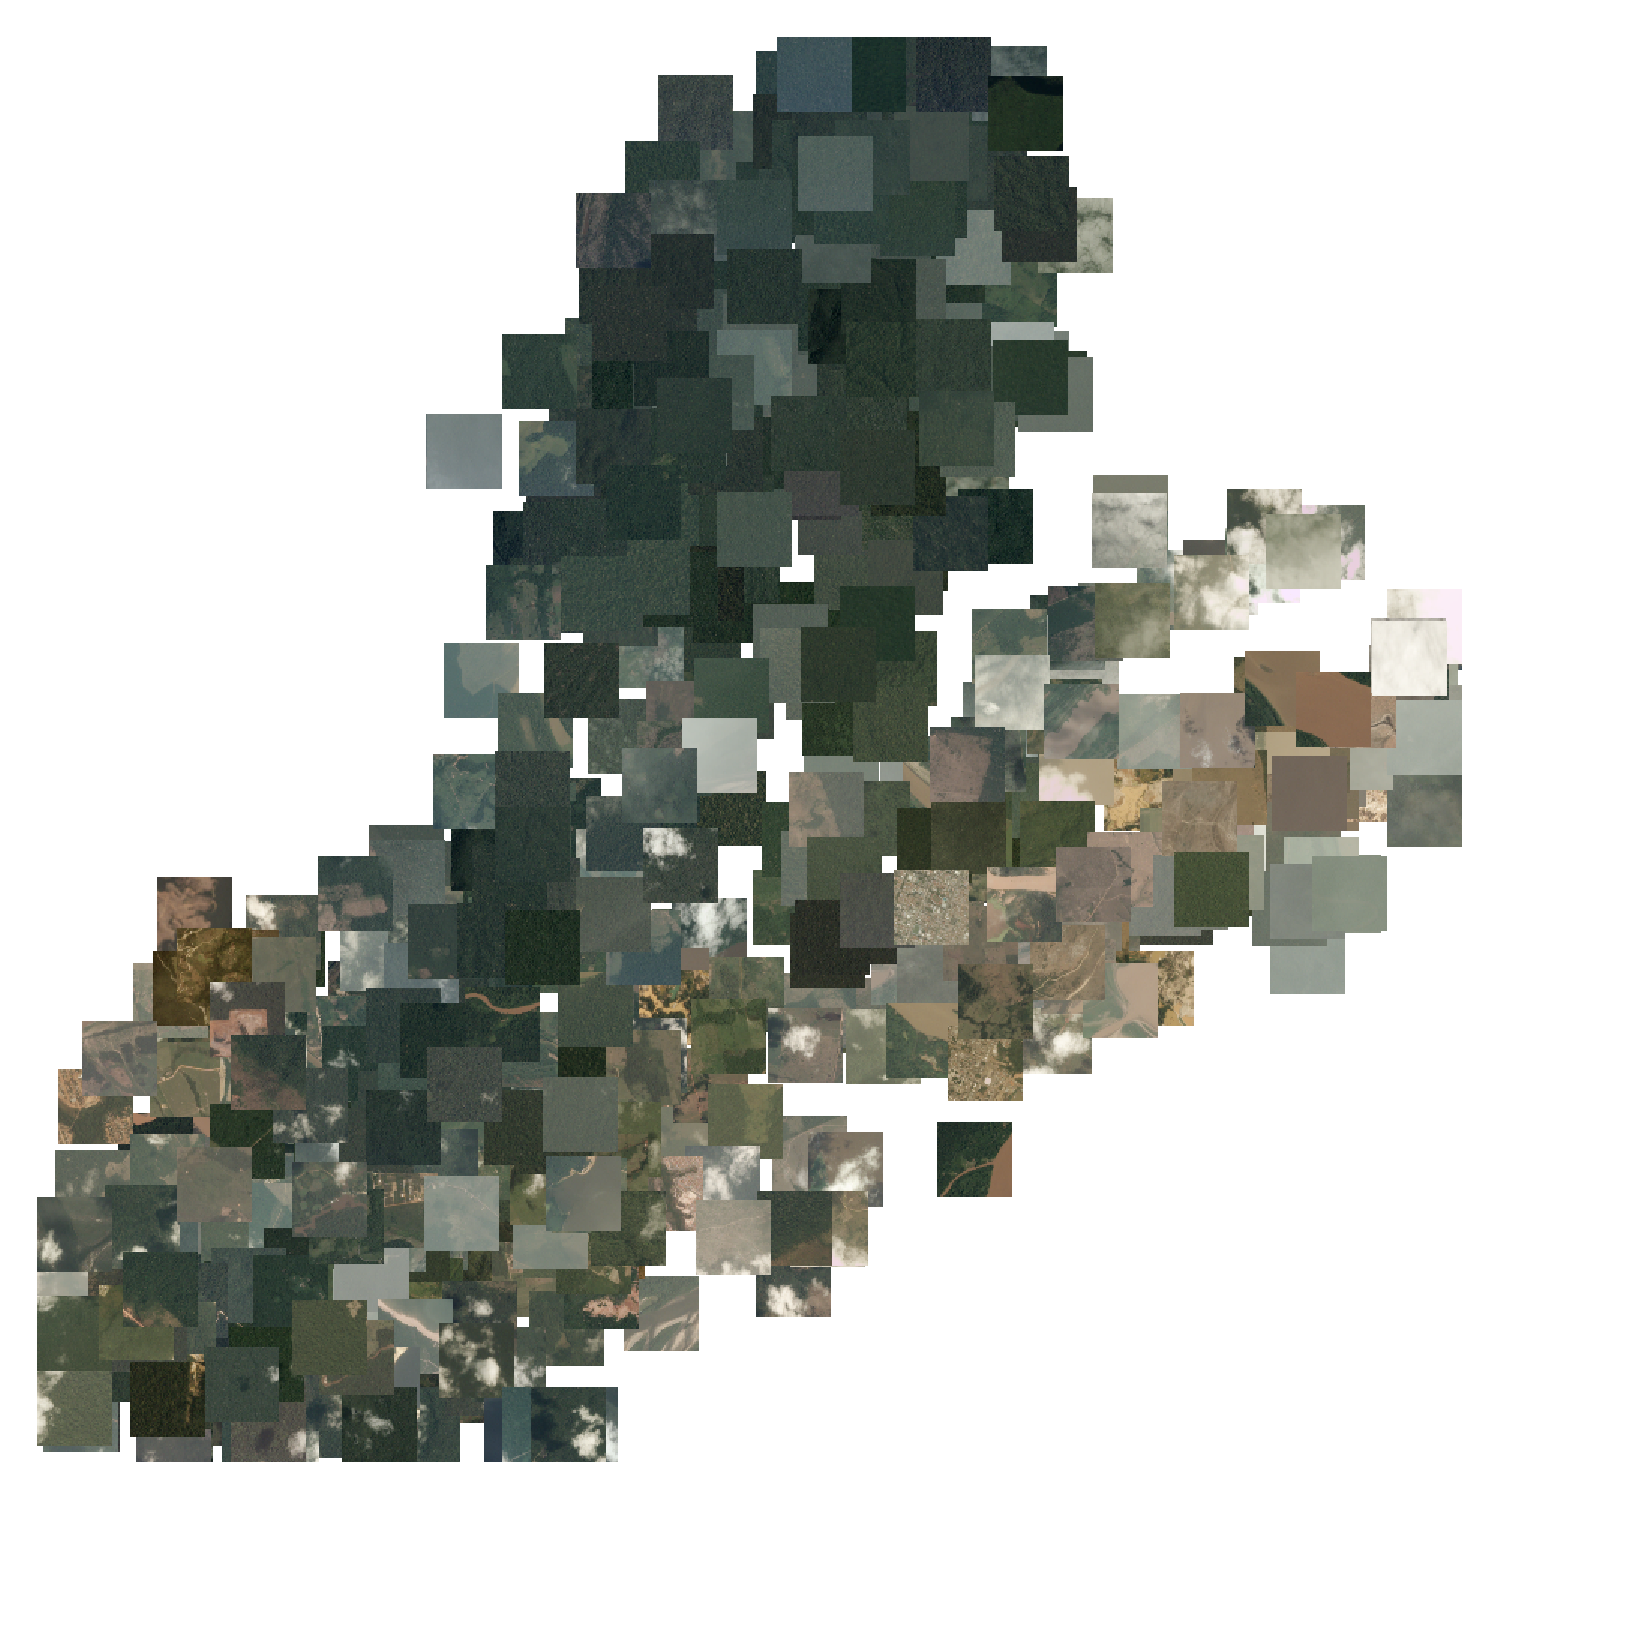
\includegraphics[width=0.7\columnwidth]{Imagens/results/rsp-resnet-50_planet_pt/TSNE Clustering.pdf}
        \caption{Agrupamento de amostras via técnica TSNE.
        Fonte: Autor}
       \label{fig:TSNE}
    \end{figure}    
\end{frame}

\begin{frame}{Pré-processamento, Transformação e carregamento}
    \begin{enumerate}
        \item   Carregamento dos canais RGB e descartando o de infravermelho-próximo de cada imagem.
        \item   Redimensionamento usando interpolação linear de $256 \times 256px$ para $224 \times 224px$. Isto se deve ao fato dos modelos já terem sido pré-treinados e configurados para essa dimensão de entrada.
        \item   Conversão da imagem para estrutura de dados numérica de Tensor
        \item   Aplicar espelho vertical ou horizontal, cada um com probabilidade de 25%.
        \item   Normalizar cada canal de cor RGB usando normalização Gaussiana com médias e desvio padrão do dataset ImageNet.
    \end{enumerate}    
\end{frame}

\begin{frame}{Definição do modelo}

\centering
\fontsize{6pt}{7pt}\selectfont
\begin{tabular}{*{8}{c}}
    \hline
    Nome & Pré-Treino & Resolution & Acurácia@1 & Acurácia@5 &  Parâmetros & FLOPs \\
    \hline
    Swin-T & ImageNet-1K & 224x224 & 81.474 & 95.5 &	28.3M &	4.5G \\
    Resnet50 & ImageNet-1K & 224x224 &	80.858 & 92.9 &	25.5M &	4.1G \\
    % https://pytorch.org/vision/main/models/generated/torchvision.models.swin_t.html
    \hline
\end{tabular}

\begin{figure}[!ht]
    \centering
    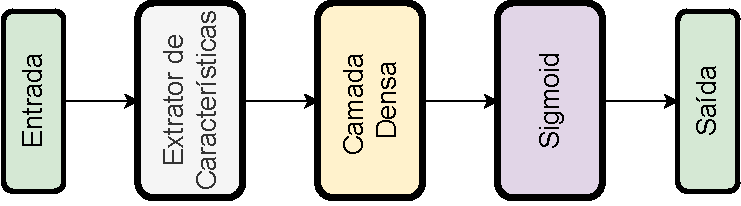
\includegraphics[width=0.7\columnwidth]{Imagens/diagrama camadas modelo.pdf}

    \caption{ Definição do modelo.}

\end{figure}  
\end{frame}


\begin{frame}
\frametitle{Seleção de modelos}
\begin{enumerate}
    \item Pesos pré-treinados
    \item Aumentar capacidade da rede
    \item Adicionar regularização 
    \item Amostrador
    \item Aumento de dados aleatória
    \item Função de perda
    \item Otimizador
    \item Taxas de aprendizado
    \item Transferência de aprendizado vs Fine Tune
    \item Experimentar os mesmos passos para o modelo Swin-T
\end{enumerate}
\end{frame}



\begin{frame}
\frametitle{Treino e validação - Modelo base}


\begin{figure}[!ht]
    \centering
    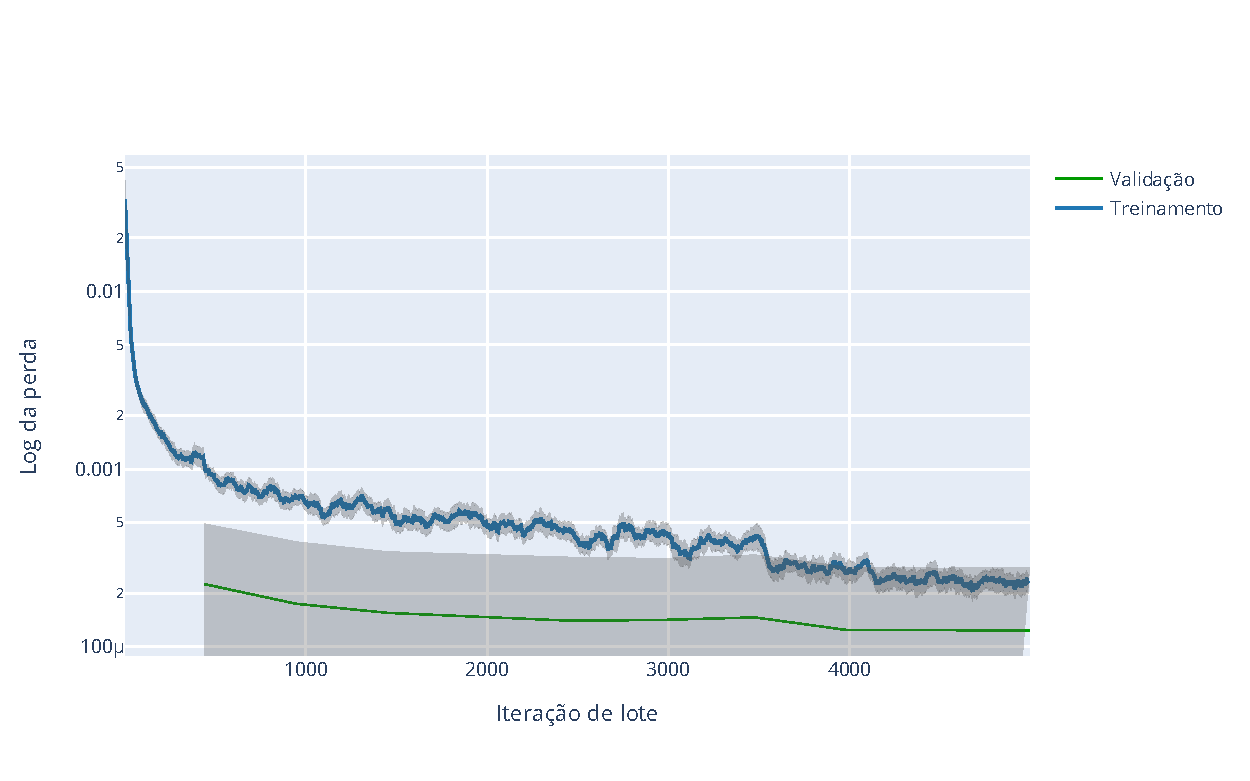
\includegraphics[width=0.55\columnwidth]{Imagens/results/rsp-resnet-50_planet_pt/Training Loss Per Minibatch.pdf}
    %\caption{ Métrica de perda em treino e validação por época para a rede ResNet50. Fonte: Autor}
    \label{fig:TreinoResnetPerda}
    \centering
    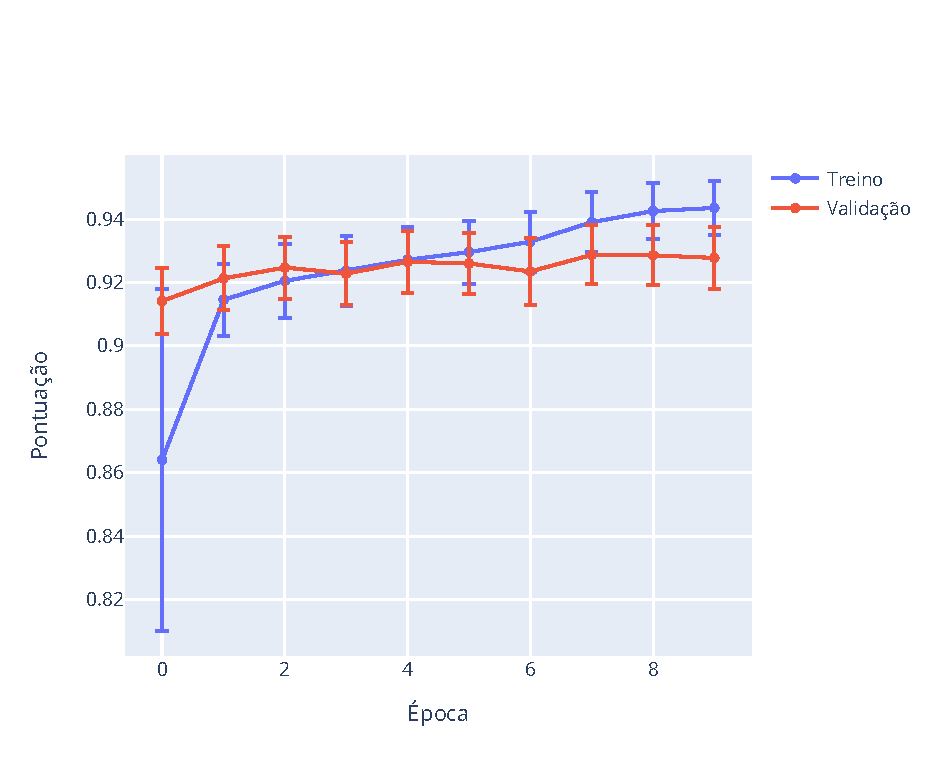
\includegraphics[width=0.40\columnwidth]{Imagens/results/rsp-resnet-50_planet_pt/Pontuação em treino e validação por época.pdf}
    \caption{ Métrica de perda e F2 em treino e validação por época para a rede ResNet50.}
    \label{fig:TreinoResnetScore}
\end{figure}  

\end{frame}


\begin{frame}{Treino e validação - Modelo proposto}    
\begin{figure}[!ht]
    \centering
    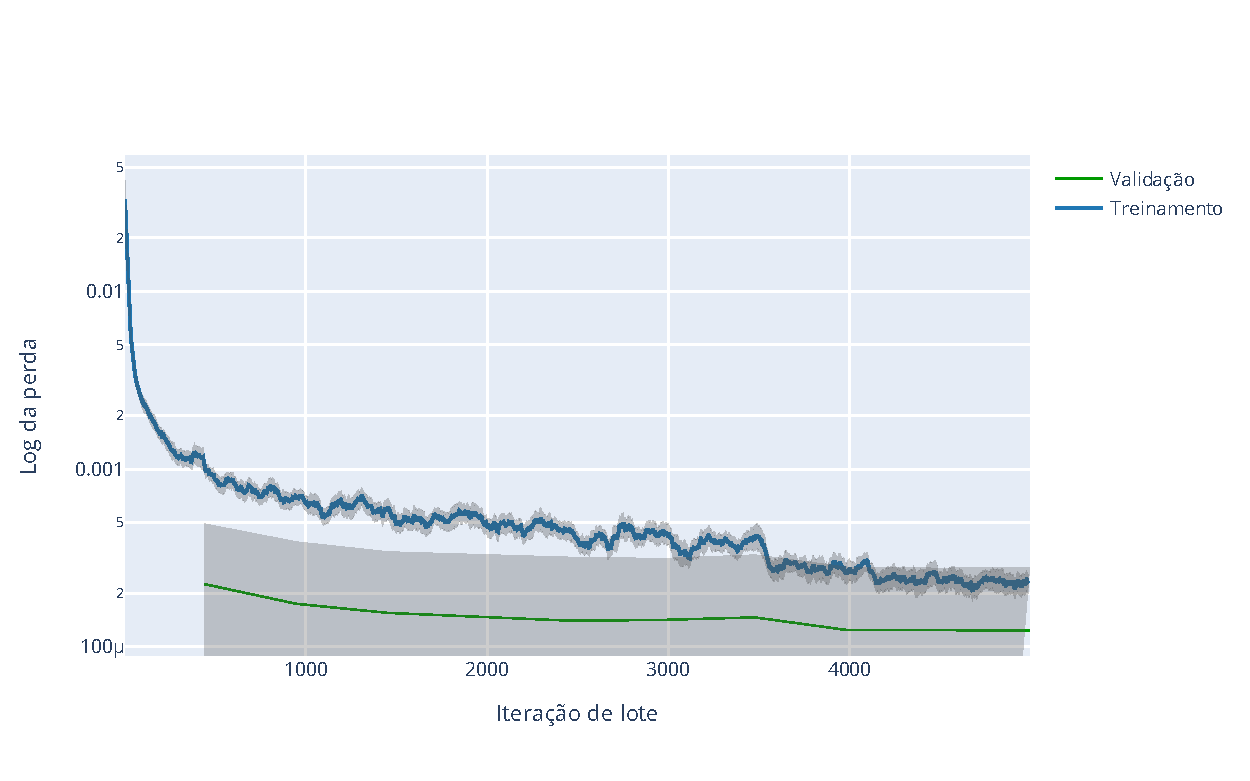
\includegraphics[width=0.55\columnwidth]{Imagens/results/rsp-resnet-50_planet_pt/Training Loss Per Minibatch.pdf}
    %\caption{ Métrica de perda em treino e validação por época para a rede ResNet50. Fonte: Autor}
    \label{fig:LossTrainSwin}
    \centering
    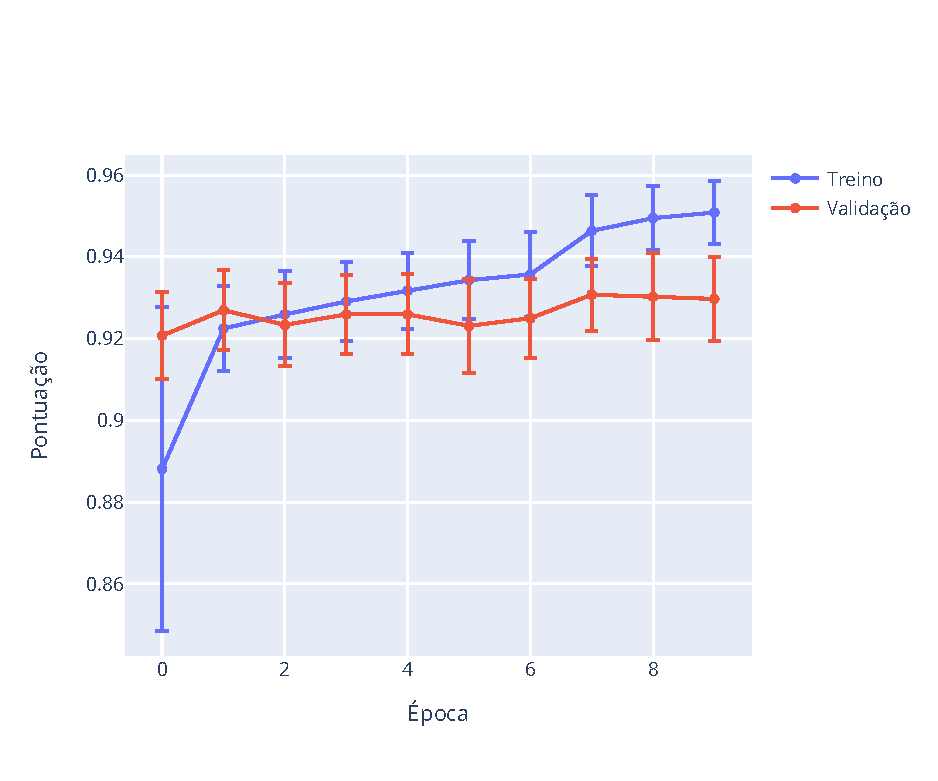
\includegraphics[width=0.40\columnwidth]{Imagens/results/rsp-swin-t_planet_pt/Pontuação em treino e validação por época.pdf}
    \caption{ Métrica de perda e F2 em treino e validação por época para a rede Swin-T.}
    \label{fig:PontuacaoTrainSwin}
\end{figure}  

\end{frame}



\begin{frame}{Resultados Modelo base - Matriz Confusão}
    \begin{figure}[!ht]
        \centering
        \includegraphics[height=0.8\textheight]{Imagens/results/rsp-resnet-50_planet_pt/Matrizes confusão.pdf}
        \caption{ Matriz Confusão para o modelo base Resnet-50. Fonte: Autor}
        \label{fig:Matriz Confusao Resnet50}
    \end{figure}     
\end{frame}     


\section{Resultados} 
\begin{frame}{Resultados do Modelo base}
    \centering
    \fontsize{6pt}{7pt}\selectfont
    \begin{tabular}{*{6}{c}}
        \hline
        {} &              Rótulo &  F2    &  Limiar   &  PR AUC &  AUC Ingênuo \\
        \hline
        15 &         slash burn &  0,030 &      0,230 &   0,145 &       0,005 \\
        3  &           blooming &  0,140 &      0,130 &   0,096 &       0,008 \\
        4  &          blow down &  0,268 &      0,190 &   0,245 &       0,003 \\
        2  &        bare ground &  0,373 &      0,210 &   0,316 &       0,024 \\
        14 &  selective logging &  0,422 &      0,090 &   0,401 &       0,010 \\
        7  &  conventional mine &  0,579 &      0,170 &   0,536 &       0,002 \\
        8  &        cultivation &  0,674 &      0,130 &   0,650 &       0,114 \\
        9  &         habitation &  0,769 &      0,130 &   0,802 &       0,093 \\
        10 &               haze &  0,774 &      0,210 &   0,784 &       0,063 \\
        16 &              water &  0,836 &      0,210 &   0,892 &       0,181 \\
        1  &     artisinal mine &  0,840 &      0,190 &   0,880 &       0,008 \\
        13 &               road &  0,864 &      0,210 &   0,916 &       0,200 \\
        0  &        agriculture &  0,890 &      0,250 &   0,929 &       0,306 \\
        6  &             cloudy &  0,910 &      0,230 &   0,946 &       0,051 \\
        11 &      partly cloudy &  0,938 &      0,210 &   0,972 &       0,173 \\
        5  &              clear &  0,978 &      0,210 &   0,996 &       0,713 \\
        12 &            primary &  0,992 &      0,190 &   0,999 &       0,928 \\
        17 &             global &  0,928 &      0,188 &   0,677 &       0,170 \\
        \hline
    \end{tabular}    
\end{frame}  


        
\begin{frame}{Classes Raras}
    \fontsize{7pt}{8pt}\selectfont
    \center
    \begin{tabular}{*{4}{c}}
        \hline
        Classe                  &            Rótulo &  Amostras      &  Proporção (\%) \\
        \hline
        Mina Convencional       & conventional mine &        100     &       0,247 \\
        Roça de Ventos          &         blow down &        101     &       0,250 \\
        Queimada                &        slash burn &        209     &       0,516 \\
        Florescimento           &          blooming &        332     &       0,820 \\
        Garimpo                 &    artisinal mine &        339     &       0,837 \\
        Desmatamento Seletivo   & selective logging &        340     &       0,840 \\
        Área Descoberta         &       bare ground &        862     &       2,129 \\
        Todo conjunto de dados  &            global &        40479   &       100.0 \\
        \hline
    \end{tabular}    
\end{frame}        
    
\subsection*{Modelo Base}
\begin{frame}{Curva PR}
\begin{figure}[!ht]
    \centering
    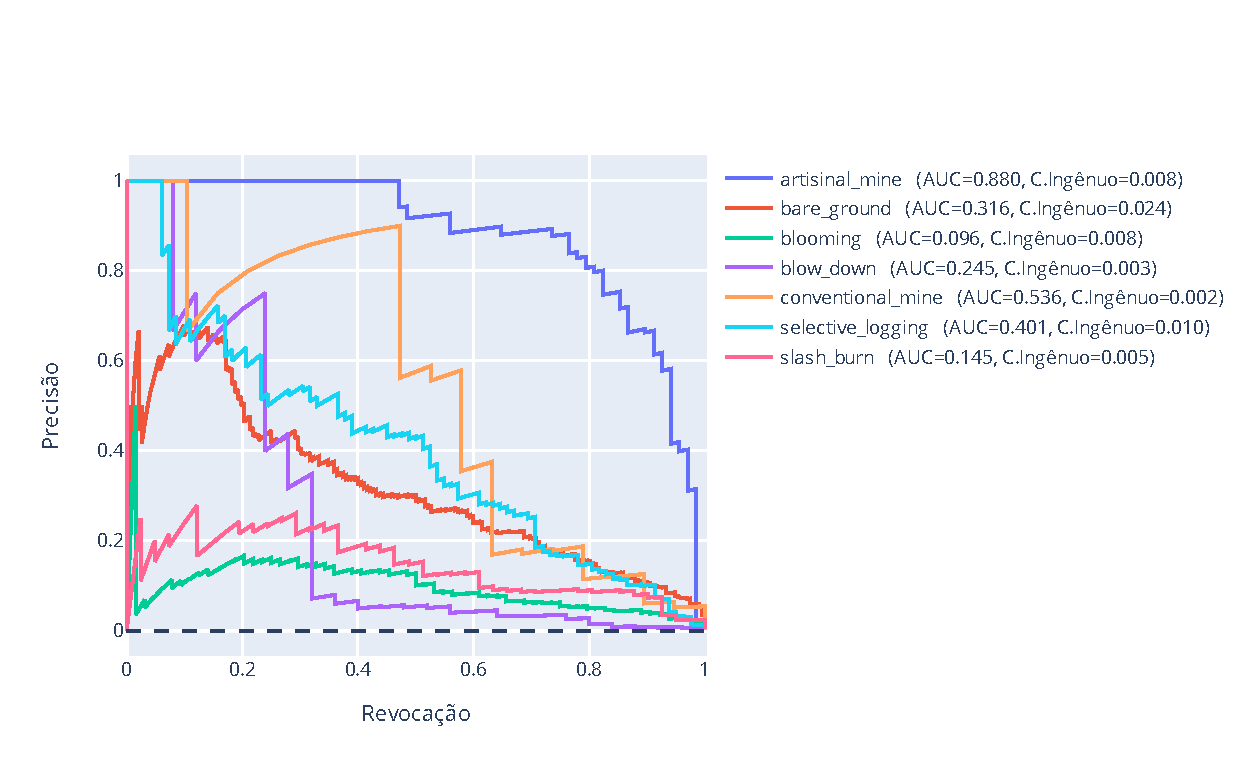
\includegraphics[width=\columnwidth]{Imagens/results/rsp-resnet-50_planet_pt/Curva PR para classes raras.pdf}
    \caption{ Curva PR para o modelo base. Fonte: Autor}
   \label{fig:CurvaPRResnet50}
\end{figure}     
\end{frame}


\begin{frame}{Resultados modelo proposto}
    \fontsize{7pt}{8pt}\selectfont
    \centering    
    \begin{tabular}{*{6}{c}}
        \hline
                     Rótulo &  F2    &   PR AUC &  PR-AUC Class.Ingênuo \\
        \hline
                  blooming &  0,230 &    0,129 &       0,008 \\
                slash burn &  0,338 &    0,342 &       0,005 \\
                 blow down &  0,310 &    0,279 &       0,003 \\
               bare ground &  0,447 &    0,344 &       0,024 \\
         selective logging &  0,475 &    0,422 &       0,010 \\
         conventional mine &  0,538 &    0,625 &       0,002 \\
            artisinal mine &  0,872 &    0,880 &       0,008 \\
                    global &  0,930 &    0,704 &       0,170 \\
        \hline
    \end{tabular}
\end{frame}     


\begin{frame}{Resultados e discussão}
    \begin{figure}[!ht]
        \centering
        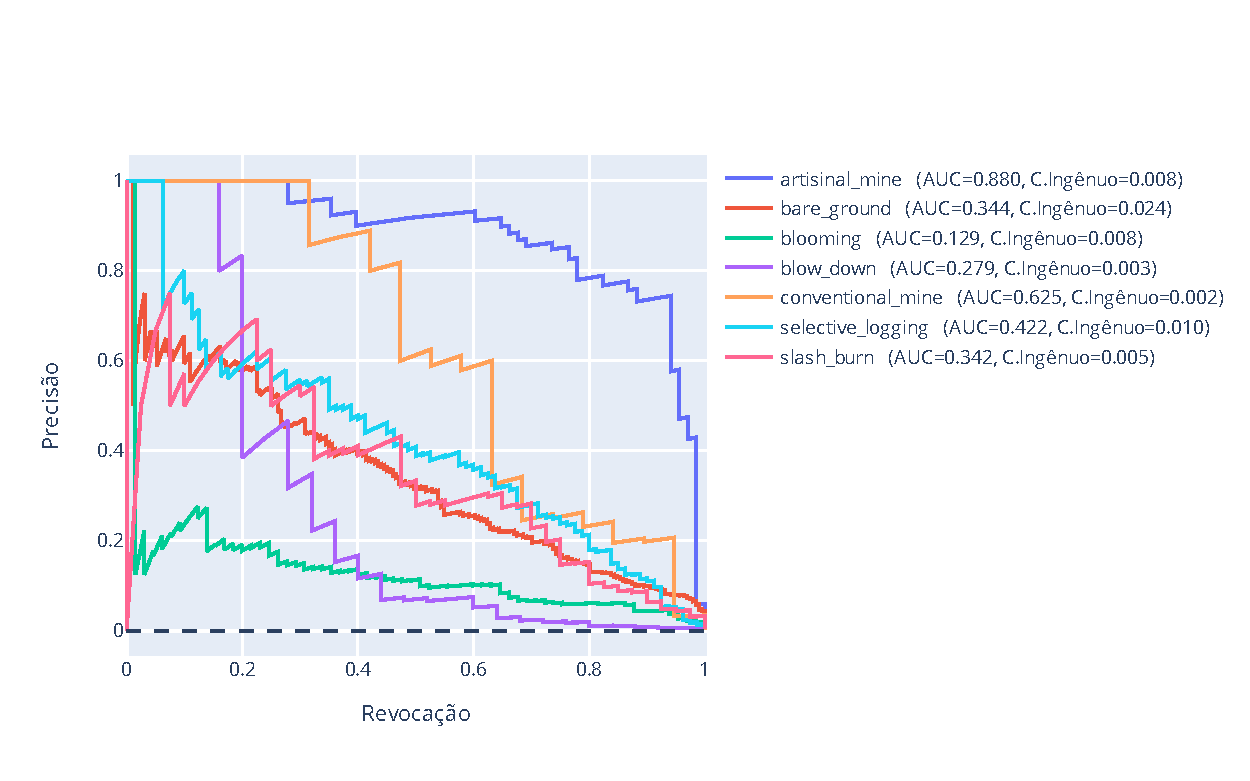
\includegraphics[width=\columnwidth]{Imagens/results/rsp-swin-t_planet_pt/Curva PR para classes raras.pdf}
        \caption{ Curva Precisão-Revocação para o modelo proposto. Fonte: Autor}
        \label{fig:CurvaPRSwint}
    \end{figure}       
\end{frame}  



\begin{frame}{Comparação de resultados}
    \centering
    \begin{tabular}{*{6}{c}}
        \hline
        Rótulo &F2-Resnet&F2-SwinT \\
        \hline
                slash burn &  0,030 &  0,338 \\ 
                  blooming &  0,140 &  0,230 \\
                 blow down &  0,268 &  0,310 \\
               bare ground &  0,373 &  0,447 \\
         selective logging &  0,422 &  0,475 \\
         conventional mine &  0,579 &  0,538 \\
            artisinal mine &  0,840 &  0,872 \\
                    global &  0,928 &  0,930 \\
        \hline
    \end{tabular}    
\end{frame}    

\begin{frame}{Resultados e discussão}
    \begin{tabular}{*{6}{c}}
        \hline
        Rótulo &PR-AUC-ResNet&PR-AUC-SwinT&PR-AUC Class.Ingênuo \\
        \hline
                slash burn &       0,145 &      0,342 &     0,005 \\
                  blooming &       0,096 &      0,129 &     0,008 \\
                 blow down &       0,245 &      0,279 &     0,003 \\
               bare ground &       0,316 &      0,344 &     0,024 \\
         selective logging &       0,401 &      0,422 &     0,010 \\
         conventional mine &       0,536 &      0,625 &     0,002 \\
            artisinal mine &       0,880 &      0,880 &     0,008 \\
                    global &       0,677 &      0,704 &     0,170 \\
        \hline
    \end{tabular}    
\end{frame}    


\begin{frame}{Resultados e discussão}
    \begin{figure}[!ht]
        \centering
        %\caption{ Probabilidade de inferência para cada classe.        Fonte: Autor}
        \includegraphics[width=0.7\textheight]{Imagens/results/rsp-swin-t_planet_pt/Inferência para cada classe.pdf}
        \label{fig:InferenciaClassesSwin}
    \end{figure}    
\end{frame}    




\section{Conclusão} 
\begin{frame}{Conclusão}
    \begin{itemize}
        \item Sensoriamento remoto
        \item Aprendizado profundo
        \item Metodologia para desenvolvimento de novos modelos
        \item Redes CNN vs Transformers
        \item Prova de conceito 
    \end{itemize}
%Este trabalho primeiro realizou um teórico sobre o sensoriamento remoto e aprendizado de máquina profundo, citando tanto conceitos fundamentais, como pontos onde as redes CNNs não apresentam bom desempenho, visando a criar um modelo aplicável á detecção de áreas irregulares como de garimpo e queimadas. Apresentou novas arquiteturas de outro paradigma de redes neurais. Contribuiu fornecendo a metodologia e aspectos necessários para realizar experimentos análogos.

%Também Foi possível realizar uma prova de conceito onde a arquitetura Swin é aplicável para o contexto de sensoreamento remoto para detecção de cenas.  Teve como ponto de partida um dataset da bacia da floresta amazônica com cenas de eventos comuns e raros e uma busca de metodologia para problemas análogos. Obteve-se um modelo baseado na arquitetura SWIN de melhor pontuação global e de principalmente nas classes raras, que indicou melhor capacidade de generalização sobre classes com poucas amostras aos já estabelecidos redes convolucionais residuais.

%Embora não tenha sido possível realizar a mesma comparação com outros conjuntos de dados, como o já mencionado Amazon Ponds, pode-se demonstrar que o modelo obtido além de compatível para esse problema, consegue superar em métricas significativas arquiteturas já estabelecidas, sendo um forte arquitetura candidata para futuros sistemas de sensoriamento remoto.
    
\end{frame}    

\begin{frame}{Trabalhos futuros}
    \fontsize{7pt}{8pt}\selectfont
\begin{itemize}
    \item Visualização e explicabilidade do o extrator de características
    \item Outros datasets para validação das conclusões
    \item Embutir em uma aplicação
    \item Perda Hamming, adequada para classificações multi-rótulos.
    \item Geração de dados sintéticos para classes raras utilizando ruido gaussiano.
    \item Canal de infravermelho próximo
\end{itemize}
\end{frame}

\section{Referências} 
\fontsize{6pt}{7pt}\selectfont
\bibliography{Referencias}


\end{document}


\begin{bibunit}[apalike]
    \fontsize{6pt}{7pt}\selectfont
    \begin{frame}{CP-nets \cite{Boutilier04a}}
      \begin{exampleblock}{Example}
        ...
      \end{exampleblock}
  
      \begin{itemize}
      \item \textbf{CP-nets}: $a: b \triangleright \overline{b}$;
      \item whereas we want: $a: b \triangleright c$.
      \end{itemize}
      \vfill
      \biblio{partage}
    \end{frame}
  \end{bibunit}

